\documentclass[12pt]{article}
%\documentclass[12pt,twoside]{report}  % For two-sided numbering
\usepackage{multicol}
\usepackage{caption}
\usepackage{csuthesis.2011}  
\usepackage{amssymb}
\usepackage{amsfonts}
\usepackage{amsthm}
\usepackage{amsmath}
\usepackage{graphicx}
\usepackage{natbib}
\usepackage[framed,numbered]{mcode}
% If you have additional pacakages to include, try including
% them prior to the above packages (especially before the 
% style file) so as to help prevent breaking the template.
% Experiment as necessary.



%%%%%%%%%%%%%%%% MACROS GO HERE %%%%%%%%%%%%%%%%%%%%%%%
%%%%%%%%%%% NO REASON TO EDIT THESE %%%%%%%%%%%%%%%%%%%
\newtheorem{theorem}{Theorem}[section]
\newtheorem{lemma}[theorem]{Lemma}
\newtheorem{cor}[theorem]{Corollary}
\newtheorem{rmk}[theorem]{Remark}
\newtheorem{prop}[theorem]{Proposition}
\newtheorem{example}[theorem]{Example}
\newtheorem{dfn}[theorem]{Definition}
\newtheorem{ass}[theorem]{Assumption}
\newcommand{\C}{{\mathbb C}}
\newcommand{\D}{{\mathbb D}}
\newcommand{\R}{{\mathbb R}}
\newcommand{\RR}{{\mathbb R}}
\newcommand{\N}{{\mathbb N}}
\newcommand{\Ss}{{\mathbb S}}
\newcommand{\V}{{\mathbb V}}
\newcommand{\X}{{\mathbb X}}
\newcommand{\Y}{{\mathbb Y}}
\newcommand{\Z}{{\mathbb Z}}
\newcommand{\ZZ}{{\mathbb Z}}
\newcommand{\rank}{{\rm rank}}

%%%%%%%%%%%%%%%%% STUDENT! %%%%%%%%%%%%%%%%%%%%%%%%%%%%%%%%%%
%%%%%%%%%%%%%%%%% Fill in Here %%%%%%%%%%%%%%%%%%%%%%%%%%%%%%

\title{Aerosol impacts on deep convective storms in the tropics: a combination of modeling and observations}		% Title of your thesis/dissertation
\author{Rachel Lynn Storer}			% What is your name?
\degree{Doctor of Philosophy}			% What degree are you getting?
\major{Underwater Basketweaving}		% This may not be necessary
\dept{Atmospheric Science}			% Department
\school{Colorado State University}		% Name of the institution
\thesistype{Dissertation}				% Thesis or Dissertation?
\committeetype{Doctoral}			% Master's or Doctoral committee?
\graduatedate{Fall}				% Semester of graduation
\graduateyear{2012}				% Graduation year
\keywords{Keyword, keyword, keyword} 		% Keywords (not typical)
\committee=4					% How many total committee members?
\cochair=1					% How many of those are cochairs?

% CHANGE THESE TO TRUE/FALSE DEPENDING ON WHETHER YOU NEED THEM
\tablespagetrue   				% Not Required
\figurespagetrue 				% Not Required
\symbolpagefalse  				% Not Required
\symbolfile{symbols} 				% Not Required
\copyrightpagefalse				% Not Required
\sectionnumberstrue				% DO NOT TOUCH
\captiontype=1					% DO NOT TOUCH
% STUDENT!
% Fill in here again
\graphicspath{{./}}				% Path to your images (default is current directory)
\mybibname{REFERENCES}				% Name of references page
\myrefname{ref}					% The name of the reference file (w/o suffix)
\deansname{Dean Reynolds}			% Dean or department head name
\committeechair{Susan C. van den Heever}			% Advisor name
\committeecochair{Cochair}			% Cochair name
\memberB{Graeme L. Stephens} 				% Other committee member names;
\memberC{Richard H. Johnson}				%    fill these in as needed
\memberD{Richard Eykholt}
\memberE{}
\memberF{}
\degreeA{}					% In case you have extra degrees...
\degreeB{}					%    not typical
\degreeC{}
\degreeD{}

%%%%%%%%%%%%%%%%%%%%% Main Document %%%%%%%%%%%%%%%%%%%

\begin{document}

%  Version: \today  % Comment this out for final version


  \titlep			% Title page; necessary
  %\copyrightpage  		% Optional; comment out if not included
  \begin{abstract}

The neural mechanisms of reinforcement learning are becoming increasingly clear following years of exciting and intense inquiry.  However, due to their reliance on primary and secondary reward concepts, reinforcement learning theories can't account for two related facts.  One, rewarding effects are observed in the absence of primary and secondary reinforcers (e.g., novelty, information and fictive outcomes).  Two, value can be transferred by inference; no pairing is needed (e.g., stimulus generalization, optimistic firing).  These atypical, or ``cognitive rewards'', have received little direct investigation; this thesis examines then a proposed mechanism that could underlie both these facts -- by treating and modeling rewards as a kind of category, reward knowledge can be constructed and transferred (by similarity-based inference) to new situations.  Using behavioral, fMRI, and computational data, this proposal was tested.  Participants completed a stimulus-response task where classical rewards (e.g.,``Correct!'' or ``Win \$1.'') were replaced with pre-trained perceptual categories, one reward category for gains and one for losses.  The reward category for each trial was a unique, never before or again experienced examplar, distinguishing this task from higher conditioning experiments. In total, the behavioral and neural data strongly suggest that cognitive rewards are in fact categories, categories which do substantively impact fMRI-based reinforcement learning signals in the brains of the human participants.  It is then further argued that as category representations are a complete mechanistic explanation for the well established generalization of (classical) secondary reinforcers, rewards are categories -- which represents a substantial change in how rewards are conceived, and modeled: the primary, to secondary, to higher-order conditioning paradigm is incomplete, perhaps even incorrect.

\end{abstract}		% Load in abstract file
  \begin{acknowledgements}   % REQUIRED
% PUT YOUR TEXT IN HERE

I would like to first thank my advisor, Dr. Sue van den Heever, for all of her support, encouragement, and advice over the years.  I am proud to be her first student, and I know many great scientists will follow me.  I would like to extend thanks to my committee members as well.  Drs. Graeme Stephens, Richard Johnson, and Richard Eykholt have offered valuable insight and my work has been better for their input.

I need to thank several people without whom this research would not have been completed.  Steve Saleeby, thank you for the budgeting code, and for countless modeling questions answered.  Tristan L'Ecuyer, thank you for your help and insight into observational data, and for your helpful suggestions as a co-author.  Matt Lebsock, thank you for providing model data, and for helpful conversations about dealing with satellite data.  Natalie Tourville, thank you for keeping my computers working over the past few years.  All of the members of the van den Heever research group have been a great help, and I think them all for the useful conversations and the fun ones.  I need to express my gratitude to my friends and family who have supported me through this process, and haven't let a crazy, stressed out grad student scare them away.

  This work was funded by the National Science Foundation under Grant NSFATM-513 0820557.
\end{acknowledgements}
	% Comment out if not included
  %\begin{dedication}
I would like to dedicate this to...
\end{dedication}
		% Comment out if not included
  \tableofcontents 		% Puts in the ToC
  \section{General Introduction}

It has been known for many years that aerosols can impact important microphysical and dynamical properties of clouds  \citep{Twomey:1977p42,Albrecht:1989p347}; however, these effects are complicated and may depend on cloud type \citep{Seifert:2006p86,VanDenHeever:2011p7996}  and environment \citep{Khain:2008p35,Lebsock:2008p45,Fan:2009p7470,Storer:2010p8001}.  It has proven particularly difficult to understand the changes that occur in deep convective clouds (DCCs) for two main reasons: (1) the presence of ice in these clouds adds additional uncertainty to processes such as precipitation formation, and (2) DCCs can form in many types of environments in association with differing types of forcing.  Much of the research performed that has examined aerosol indirect effects on DCCs, as summarized by \citet{Khain:2009p18} and \citet{taoreview}, has had mixed results both in terms of the effect of aerosols on the precipitation produced by these clouds, as well as whether convective invigoration occurs in polluted storms.  The purpose of the work summarized here is therefore to add to the knowledge of how the presence of increased aerosols can impact DCCs, through a combination of modeling and observational analysis.

This dissertation is split into two main components.  Chapter 2 describes a modeling study undertaken in order to learn the important processes occurring in DCCs that are affected by increasing aerosol concentrations.  A series of large scale, two-dimensional model runs were completed, with only the aerosol concentration differing, and a large sample of DCCs was analyzed for aerosol effects.  The microphysical budget was examined in detail in order to distinguish which processes were important for precipitation formation and latent heating, and to examine how these processes were affected by the presence of increased numbers of aerosols.  This chapter has been submitted, in this form, as a manuscript to the Journal of Atmospheric Science, and has been accepted pending revisions.

\newpage\noindent
Up until now, no observational studies have been published in which aerosol impacts on deep convection are examined over a large spatial and temporal scale.  Other observational studies on aerosol indirect effects have focused on a very limited spatial domain, or did not isolate the impacts specifically on deep convection.  In order to evaluate whether the aerosol indirect effects described in the modeling study can be observed, a study was performed utilizing CloudSat data; this research is summarized in Chapter 3.  Four years of satellite data were analyzed in a region of the East Atlantic in keeping with the conditions simulated in Chapter 2.  A large sample of DCCs was acquired over a four year period and matched with aerosol optical depth (AOD) information obtained from a global transport model.  Four parameters (center of gravity, cloud top, rain top, and ice water path) were examined for differences associated with changes in AOD.  An attempt was made to separate out environmental effects from the effects of aerosols by splitting the data up by convective available potential energy (CAPE) and lower tropospheric static stability (LTSS), and the results were tested for significance.  This chapter is a manuscript in preparation to be submitted to a peer-reviewed journal.		% Start including your chapter files
  \section{Chapter 2 -- Task and Models} % (fold)
\label{sec:task_and_models}
This chapter has two parts, the overall aim of which is to show how a stimulus-response task was used to examine possible category representations of rewards, and then to described how learning in that task was modeled (using a set of reinforcement learning equations).  To that end, and in that order, first the behavioral task is described and its results characterized.  Second, the computational models are rigorously laid out, as are their results.

\subsection{On Task}
\label{sub:to_task}
\subsubsection{What they did, and when}
\label{subsub:whatwhen}
The behavioral task each participant completed consisted of two parts.  Depicted in Figure~\ref{fig:task}. (\emph{top}), the first was a passive learning task wherein participants learned two rewarding perceptual categories by viewing randomly selected black and white sinusoidal gratings.  Each grating (which was on-screen for 2 seconds) was followed by ``Gain \$1'' or ``Lose \$1'' in, respectively, green or red letters (1 second).  The width of the grating's lines and their angles was derived from an information integration (category) distribution (Figure~\ref{fig:II}; borrowed from \citep{Spiering:2008p5008}).  The disappearance of each grating and appearance of the reward was separated by an empty grey screen (1 second).  Each trial terminated in a fixation cross (lasting at least 0.5 seconds). In total then, each trial lasted a total of 4.5 seconds.  The trials for part 1 were spread over an initial training period completed outside the scanner, lasting 126 trials, and an in-scanner refresher lasting 45 trials.  Prior to beginning training participants were, after some preliminaries, instructed to, ``Attend to the screen in order to learn which types of gratings indicate wins and which types indicate losses''.  To minimize any stimulus specific effects, the category parameter distribution (Figure~\ref{fig:II}) to reward (i.e., ``Gain \$1'' or ``Lose \$1'') mapping was randomized for each participant.

Part 2 was a stimulus-response task that replaced classical rewards with an appropriate grating from task 1 (Figure~\ref{fig:task}, \emph{bottom}).  Gratings drawn from the Gain category were used for positive reinforcement, while gratings indicative of losses were used as negative reinforcers.   Each trial began with an abstract black and white ``tree'' stimuli (left most image in bottom of Figure~\ref{fig:task}).  Each ``tree'' deterministically belonged to one of two arbitrary response categories (``q'' or ``w'').  Subjects indicated their response by button press using either the right or left index fingers on a magnet-compatible response box.  The response window lasted up to 2.5 seconds, but ended as soon as a response was made.  Immediately following response the ``tree'' was replaced with a blank grey screen, which was on-screen for half a second and was replaced with a feedback screen.  If the response was correct a \emph{never before experienced} exemplar grating from the gain distribution was used; if the participant was incorrect, a new loss grating appeared instead.  The use of novel gratings forced the subjects to classify each grating prior to inferring its value.  This necessary inference made these rewards incompatible with primary or secondary definitions.  If no response was made, or the wrong button was pressed, the subject's reward was replaced with, ``No response detected'' (these trials were excluded from further analysis).  Feedback always lasted for 1 second and was terminated by a fixation cross (0.5 seconds).  

For the instructions in part 2 participants were told, ``Each tree belongs to either category q or w.  Which is the correct answer though is random.  The shape of trees is meaningless.  To learn the correct response for each tree you must start by guessing.  Use what you learned about the rewarding properties of the gratings from part 1 to learn the right responses.  Remember, a random subset of the Gains and Losses are real.  These mostly determine how much you'll earn for your participation.  So try and earn as much money as possible''.  Instruction for both parts were given orally by the experimenter using a script and Figure~\ref{fig:task} as a visual aid.

Over the course of part 2, participants learned to classify 6 ``trees'', randomly selected at the start of the experiment out of a pool of 22 possible.  Each of the 6 were experienced a total of 28-32 times for a total of 199 trials. The order of the trials in the second half of part 1 and all of part 2 was determined using a genetic algorithm designed to optimize fMRI signal detection, among other considerations.  Most relevant to behavioral analysis, trials were in pseudo-random order with second order counterbalancing.  For remaining details see p\pageref{sub:acquired}.

As part of fMRI data acquisition, 18 participants completed both parts of the task (10 female, mean age of 24, ranging from 21 to 32). Participants were compensated at a base rate of \$15.00 earning up to \$30 more depending on behavioral performance. For the last 30 trials the participant was paid an additional dollar for every correct response and lost a dollar for every incorrect response.  Before beginning experiment participants were told that some trials would count, but were not told until after which trials (i.e., the last 30).  The highest payout was \$45, i.e.,perfect performance, the lowest was 30, indicating near chance behavior for the last 30.  The average payout was \$40.23.

Of the 18 participants, two were removed all analyses as they demonstrated inverse learning (Figure~\ref{fig:sacc}, see \emph{107} and \emph{110}).  Despite reporting a full understanding of the reward contingencies from part 1, in part 2 these participants displayed significant and consistent decreases in performance through time.  Had this learning been in the usual direction it would have been considered better than average performance.  In post task interviews both reported feeling as if they performed above average.  Once they were informed of their inverse performance neither believed it.  It seems possible then that both correctly learned the perceptual characteristics but mis-mapped the value labels, i.e., they got ``Gain'' and ``Loss''  mixed up.  Post-experiment interviews further suggested that both the discarded subjects were under high personal stress.  One subject, who was a PhD student, had his competency exams the next day.  The other completed a 60 mile bike ride an hour prior to participation.  Combined these participant's data suggest that the perceptual and verbal characteristics of the reward categories are independently accessible, and that the verbal label may be more labile than the perceptual distributions.  However given the other participants consistent positive performance and rapid learning it seems these two were a curious but isolated anomaly (Figure~\ref{fig:sacc}).

\begin{figure}[tp]
    \noindent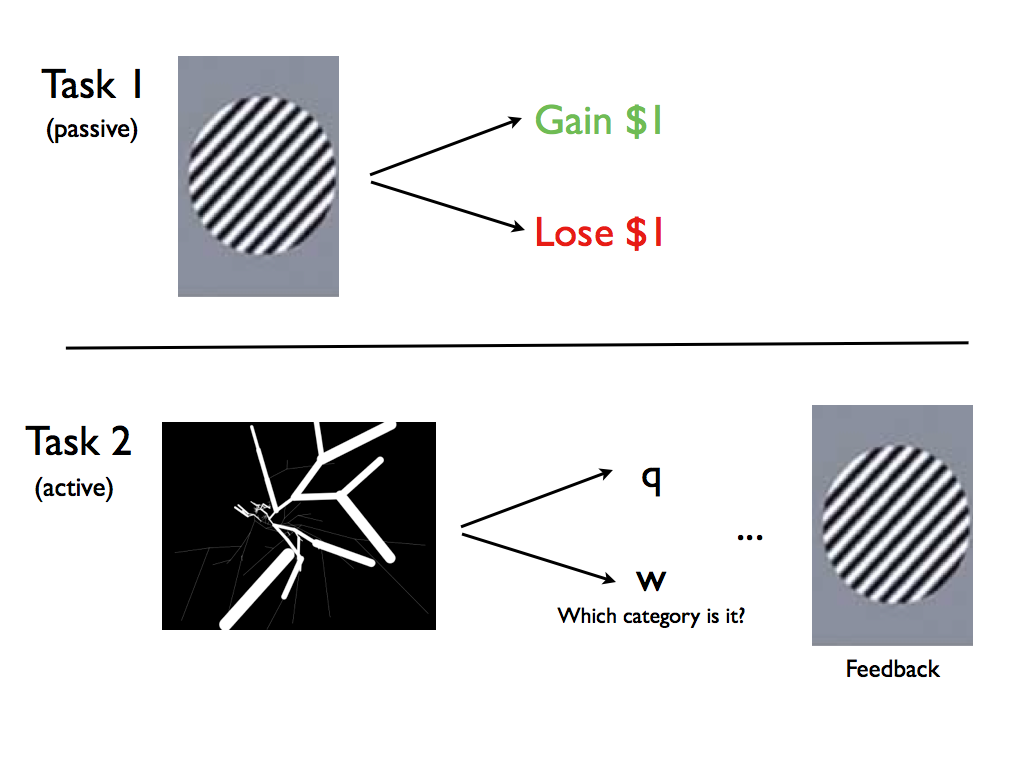
\includegraphics[width=39pc]{f_task}
    \centering
    \caption{Depiction of the behavioral task.  The \emph{top} depicts part 1, the passive learning of the reward categories.  The \emph{bottom} depicts part 2, the stimulus-response learning phase.}
    \label{fig:task}
\end{figure}

\begin{figure}[tp]
    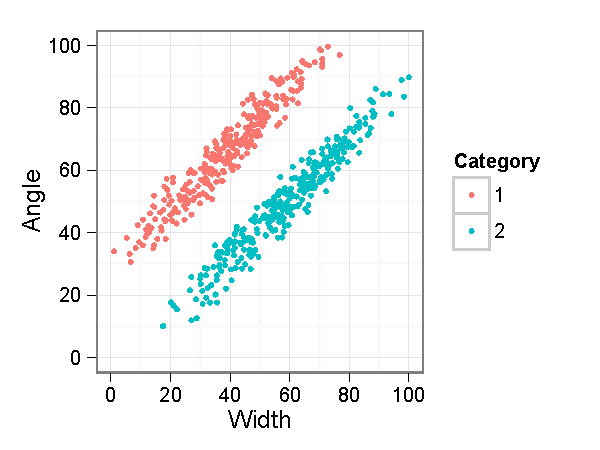
\includegraphics{f_II}
    % TODO -- replace with the good plot; find the good plot again.
    \centering
    \caption{The two sinusoidal grating distributions for the information integration (II) category distributions.   As II categories span the diagonal of the gratings parameter space (line width and angle successful learning requires consideration of both dimensions preventing participants from solving the categorization problem with simple rule-based strategies.}
    \label{fig:II}
\end{figure}

\begin{figure}[tp]
    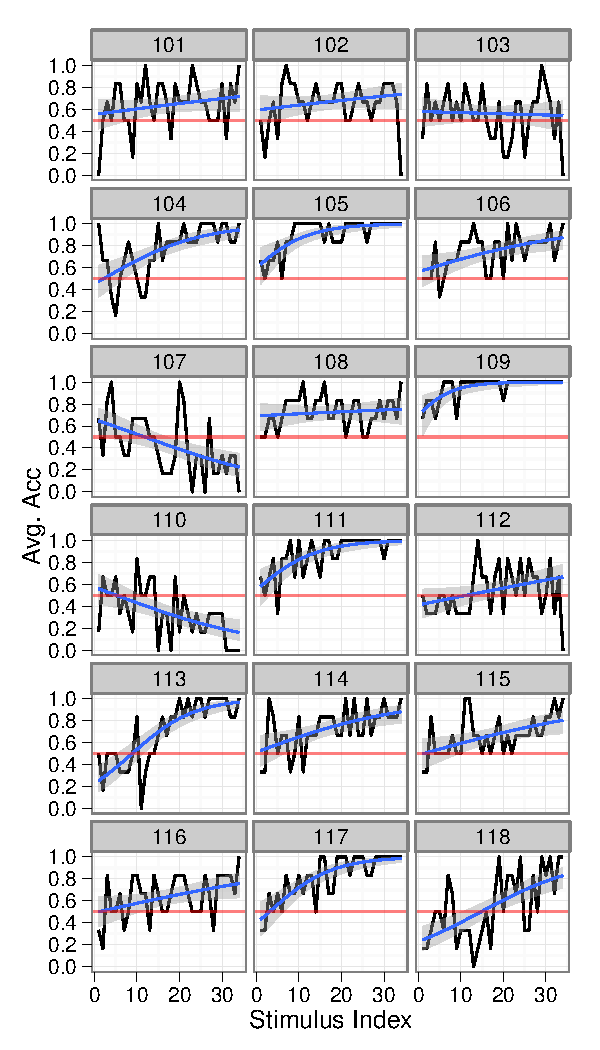
\includegraphics{f_all_sS_acc}
    \centering
    \caption{Average accuracy for each participant (black), averaged for all 6 stimuli by trial (i.e., Stimulus Index), blue line and the grey area represent a binomial regression fit of the data and bootstrapped 95\% confidence intervals, respectively.}
    \label{fig:sacc}
\end{figure}

\begin{figure}[tp]
    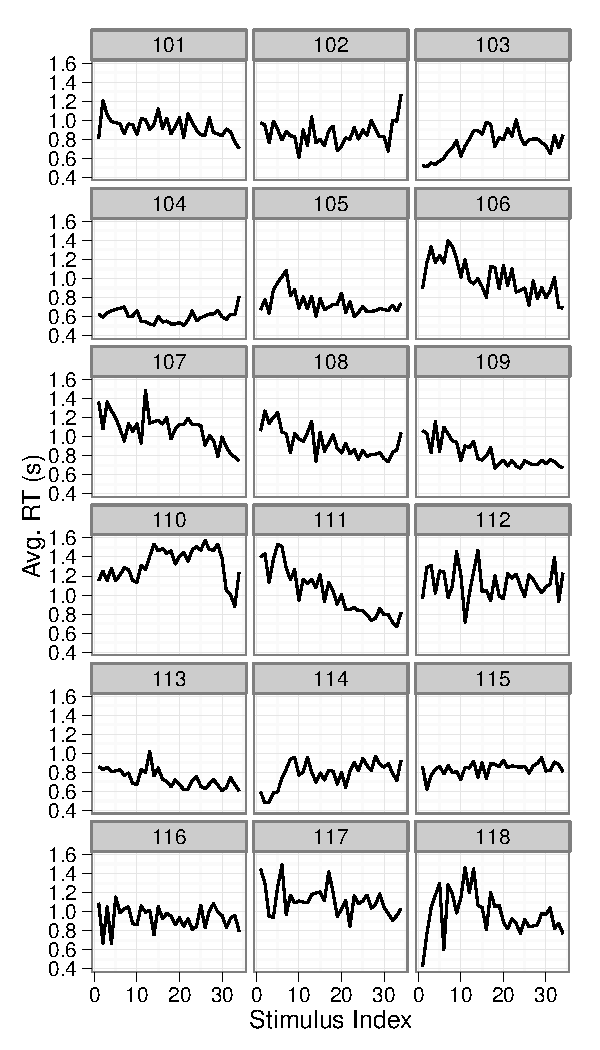
\includegraphics{f_all_sS_rt}
    \centering
    \caption{Mean reaction time for each participant, averaged for all 6 stimuli by trial (i.e., Stimulus Index).}
    \label{fig:srt}
\end{figure}

\subsubsection{Well behaved results}
\label{subsub:wellbehaved}
On an individual basis the lower confidence interval\footnote{All confidence intervals were bootstrapped estimates calculated suing the Hmisc package (\url{http://cran.r-project.org/web/packages/Hmisc/index.html}) in the R programming language (v2.15.1; \url{http://www.r-project.org/})} around the binomial fit of the accuracy data rose to above the chance level (0.5) by the last trial, except for participant 103, who did not learn (Figure~\ref{fig:sacc}).  Many participants (11 of 16) greatly exceeded this minimum criterion, showing above chance learning by trial 10, and nearly all (14 of 16) exceeded chance by trial 20  (Figure~\ref{fig:sacc}).  These individually good performances are reflected in the participants' aggregate performance, which was well above chance by trial 5 (Figure~\ref{fig:meanacc}).  This aggregate learning rate is consistent with past work in the lab using verbal or monetary feedback \citep{Seger:2010p7188,Seger:2005pd}, as it is with other results in other laboratories \citep{ODoherty:2003p6329,Ramnani:2000p6515,Aron:2004p1375,Smith:2008p2803,Poldrack:2008p6839,Ashby:2006p9153,Ashby:2005p4764,Ashby:2005p9152}, indicating that the rewarding categories in present study are behaviorally similar to classical rewards.  The consistency between classical rewards and this task were also reflected in the reaction time measures, which showed a 200 ms decrease over time, bottoming out near 850 (for individual averages see Figure~\ref{fig:srt} and for overall performance see Figure~\ref{fig:meanrt}).  Responses in similar, classically rewarding tasks end with reaction times near 700-800 milliseconds and show similar rates of decline.  The 50-100 ms possible difference in reaction times may be due to the increased difficultly of classifying the rewards compared to simply reading the value of the outcome (e.g., ``Gain \$1'').

\begin{figure}[tp]
    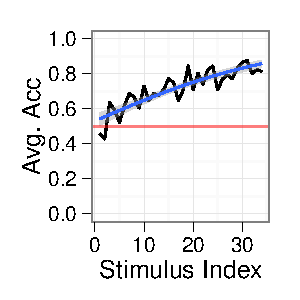
\includegraphics{f_all_mean_acc}
    \centering
    \caption{Mean accuracy (black), averaged over all participants and stimuli, plotted by trial.  The blue line and grey area represent a binomial regression fit of the data and bootstrapped 95\% confidence intervals, respectively.}
    \label{fig:meanacc}
\end{figure}

\begin{figure}[tp]
    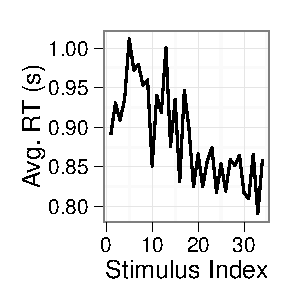
\includegraphics{f_all_mean_rt}
    \centering
    \caption{Mean reaction time (black), averaged over all participants and stimuli, plotted by trial.  The blue line and grey area represent a binomial regression fit of the data and bootstrapped 95\% confidence intervals, respectively.}
    \label{fig:meanrt}
\end{figure}

\subsection{3 Models and 2 Codes}
\label{sub:threemodels}
\subsubsection{Our three models}
\label{subsub:catquant}
Three Rescorla-Wagner-like models were constructed, each using a distinct reward representation.  The first model treated rewards identically to a classical reward (e.g., a 0 for a loss or 1 for a gain).  The second and third devalued each reward based on how similar it was to the category mean.  This similarity metric is (necessarily) simplistic.  As was reviewed on p\pageref{subsub:curves}, there are many proposed models for how the categories are represented.  Likewise, our understanding of the computational implementation of the category learning systems is only just underway \citep{Ashby:2005p9152,Ashby:2006p9153}.  As such there is no obvious way to interlace the hypothesis of rewarding categories with the category learning systems or with the many models of categorization they rely on.  Avoiding such ambiguity, a simpler route driven by Shepard's basic finding \citep{Shepard:1987p9102} was taken.  Whatever the representation and/or category learning system that (may) implement rewarding categories, Shepard's work insists they show an exponential or Gaussian decline with similarity.  For simple stimuli like a light or tone, similarity is measured from the initial training prototype \citep{Guttman:1956p8355}.  However as the task does not have a singular prototype the mean of the parameters for all training trials (i.e., part 1) was used in its place.  This simple substitution makes categories identical to the simplest of the prototype category representations \citep{Rosch:1973p9108,Ashby:1995p9109}, making this a parsimonious yet literature driven first attempt to quantify similarity of rewards.  Therefore, for model two similarity decreased exponentially measured from the training mean, while for model three it decreased following a normal Gaussian (for complete mathematical detail see p\pageref{subsub:codesandfits}).  

\subsubsection{Codes and fits}
\label{subsub:codesandfits}
For each participant and model, the two free parameters ($\alpha$, which controls each model's rate of learning and $\beta$, which controls the steepness of the action selection criterion) were fit using an exhaustive\footnote{With a 0.05 precision, ranging from 0-1 for $\alpha$ and 0-5 for $\beta$} maximum log-likelihood search.  Additionally each model was run using two separate reward coding schemes.  In the first scheme gains were valued as 1 and losses as 0.  The second, which was based on the bivalent monetary value of the rewards, uses 1 and -1 for gains and losses respectively.  The first scheme is universally used in human and animal modeling studies as well as in machine learning, and is the \citep{Sutton:1998p9247} recommended scheme.  However recent recordings of dopaminergic neurons in monkey suggest that the true reward codes are complex, even perhaps redundant \citep{Kim:2006p1063,Matsumoto:2009p7219}.  Among other schemes, they reported firing consistent with a bivalent reward code.  Using the second scheme is merely a first, albeit simple, step in incorporating the potential complexity of dopaminergic firing as observable by the fMRI BOLD signal and in human subjects.

\subsubsection{The incantations}
\label{subsub:incantations}
To restate more formally, a Rescorla-Wagner-like model's value updates were defined by,
\begin{equation} \label{eq:V} V(s_t,a_t) \leftarrow V(s_t,a_t) + \alpha\delta \end{equation} 
\begin{equation} \label{eq:rpe} \delta = r_{(classic,t)} - V(s_t,a_t) \end{equation}
where $\delta$ is the reward prediction error, $s$ is a stimulus, or state (or which there were 6), and $a$ is an action (either ``q'' or ``w'') and $r_{classic}$ (the numerical representation of the rewards) can be coded as either
\begin{equation}
    \label{eq:r1}
    r_{classic}= \{1,0\}
\end{equation}
or 
\begin{equation}
    \label{eq:r2}
    r_{classic}= \{1,-1\}
\end{equation}
but where $r_{classic}(t)$ may also be replaced with
\begin{equation}
    \label{eq:re}
    r_{exp} = r_{classic}S_{exp}
\end{equation}
or
\begin{equation}
    \label{eq:rg}
    r_{gauss} = r_{classic}S_{gauss}
\end{equation}
where $D$ is the Euclidean distance from the width ($w$) and angle ($\theta$) of that trials reward category to the average values from the pre-training ($\bar{\theta}$ and $\bar{W}$; see discussion on part 1 on p\pageref{subsub:whatwhen})
\begin{equation}
    \label{eq:D}\\
    D = \sqrt{(\bar{\theta} - \theta)^2 + (\bar{W}-w)^2}
\end{equation}
is transformed to a Shepard-like similarity metric \citep{Shepard:1987p9102}:
\begin{equation}
    \label{eq:Sexp}\\
    S_{exp} = e^{-D}
\end{equation}
\begin{equation}
    \label{eq:Sgauss}\\
    S_{gauss} = e^{-D^2}
\end{equation}
Consistent with past work, all values are initialized at 0 \citep{Beierholm:2011p8141,BischoffGrethe:2009p4570,Gershman:2009p7207}
\begin{equation} \label{eq:V0} V_{initial} = 0. \end{equation}
and values are transformed to response selection probabilities via the softmax distribution \citep{Sutton:1998p9247,ODoherty:2003p6329}.
\begin{equation}
    \label{eq:softmax}
    p_1(s_t,a_t) = {e^{\beta V_1(s_t,a_t)}\over{e^{\beta V_1(s_t,a_t)} + e^{\beta V_2(s_t,a_t)}}}
\end{equation}
where $V_1$ and $V_2$ are the values for the two response options (i.e., ``q'' and ``w'').
During maximum likelihood parameter selection (p\pageref{subsub:codesandfits}), the $p_1(s_t,a_t)$ values from each trial and some test parameters ($\alpha_{test}$ and $\beta_{test}$) calculate the log-likelihood by,
\begin{equation}
    \label{eq:logL}
    L_{} = \sum{log_e(p_1(s_t,a_t))}
\end{equation}

\subsubsection{Fits and plots}
\label{subsub:fits}
On average none of the three models fit the accuracy data better than the rest (Figure~\ref{fig:logL}).  For brevity's sake each model will be referred to as ``none'', ``exp'' and ``gauss'', corresponding to Eq~\ref{eq:rpe}, Eq.\ref{eq:re}, and Eq.~\ref{eq:rg} respectively.  Nor did the coding scheme impact the fits (``acc'' and ``gl'', matching respectively Eq.~\ref{eq:r1} and Eq.~\ref{eq:r2}; Figure~\ref{fig:logL})).  For ``acc'' the step size parameter (``alpha'' in Figure~\ref{fig:alpha} matching $\alpha$ in Eq.~\ref{eq:V}) increased in ``exp'' compared to the other models.  This increase was expected as the exponential similarity metric can sharply decrease the magnitude of each value update, requiring an increase in $\alpha$ to compensate.  A similar trend was observed for the temperature parameter (``beta'' in Figure~\ref{fig:beta}, matching $\beta$ in Eq.~\ref{eq:softmax}). The more equiprobable each action is the larger the temperature parameter.  As such the increase for ``exp'' means participant's choices are more likely to change from trial to trial, which is again consistent with a decrease in update magnitudes.

Importantly the intra-subject variability in $\alpha$ and $\beta$ was low, as demonstrated by the small standard error of both parameters (Figure~\ref{fig:alpha} and~\ref{fig:beta}).  Consistent parameter estimates between subjects support the use of subject-level parameters in the fMRI analyses, which in other hands have been reported to be too noisy to be reliable \citep{Daw:2011p7995,Seymour:2007p7585,ODoherty:2003p6329}.  Using subject-level parameters is a crucial step in assessing and maximizing model quality. The goal of any model of human behavior is to make good predictions for individual cases not just for aggregates of tens or hundreds of participants \citep{Daw:2007p9346}.  However aggregates prediction is the norm in reinforcement learning models of human behavior (for examples see, \citep{Daw:2011p7995,Seymour:2007p7585,ODoherty:2003p6329}).

\begin{figure}[tp]
    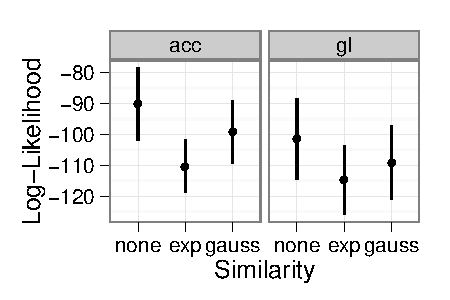
\includegraphics{f_logL}
    \centering
    \caption{Average negative log-likelihoods for each of the models and coding schemes.  Error bars represent standard errors.}
    \label{fig:logL}
\end{figure}

\begin{figure}[tp]
    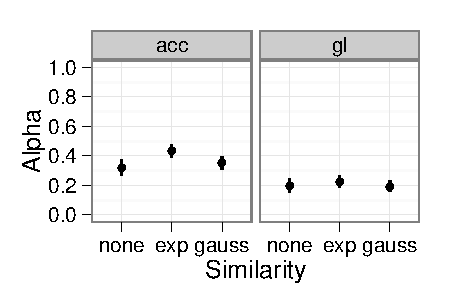
\includegraphics{f_alpha}
    \centering      
    \caption{Average alpha values for each of the models and coding schemes.  Error bars represent standard errors.}
    \label{fig:alpha}
\end{figure}

\begin{figure}[tp]
    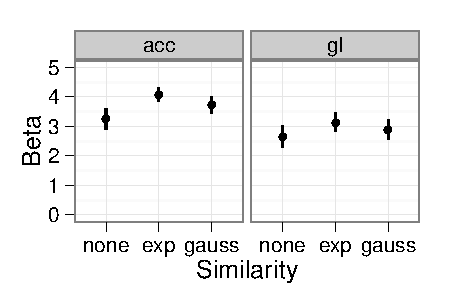
\includegraphics{f_beta}
    \centering
    \caption{Average beta values for each of the models and coding schemes.  Error bars represent standard errors.}
    \label{fig:beta}
\end{figure}

The fit reinforcement learning models for every participant and coding scheme can be found in Figure~\ref{fig:rpeacc} -~\ref{fig:valuegl}.  In the traditional formulation, where similarity does not impact reward value (e.g., see Figure~\ref{fig:rpeacc} or~\ref{fig:rpegl}) the reward prediction error decreases with learning, eventually plateauing at 0, for strong examples see subjects \emph{102}, \emph{105} and \emph{111} in the ``none'' column of Figure~\ref{fig:rpeacc}.  In contrast, both similarity models, ``exp'' and ``gauss'', never fully plateaued (again see Figure~\ref{fig:rpeacc}).  In the context of the models, this is expected.  Each grating will, in all likelihood, be non-identical to the mean. However as the parameter mean is the asymptotic expectation, reward prediction errors happen even after learning is complete.  In the big picture, this is the desired behavior.  The similarity adjusted models are trying to capture the case where a reward's value may vary in ways that are not predictable \emph{a priori}; Given the massive multiplicity of possible outcomes in the world it is unlikely to find the same one multiple times.  Small prediction error should then continue without end, as happens in these models.

When comparing ``exp'' and ``gauss'' models, you'll see the former appears to have lower magnitudes (Figure~\ref{fig:rpeacc}).  Examining density plots composed of all participants data confirms this observation (Figure~\ref{fig:denrpe}).  The density plot also reveals that ``exp'' prediction errors are diminished more rapidly than their ``gauss'' counterparts (a pattern most clearly scene in the left panel of Figure~\ref{fig:denrpe}).  

Regardless of model class, between the two reward codes there are substantial differences in reward prediction behavior.  The $\{1,-1\}$ (denoted in these plots as ``gl'') scheme leds to substantially more negative deflections that the $\{1,0\}$ scheme (``acc'') (compare Figure~\ref{fig:rpegl} and ~\ref{fig:rpeacc} as well as the \emph{left} and \emph{right} panels of~\ref{fig:denrpe}).   

Value estimates for the two similarity adjusted rewards (i.e., ``exp'' and ``gauss'') were generally less than the alternative classic model (``none'' in Figure~\ref{fig:valueacc} and~\ref{fig:valuegl}).  However, as a consequence of their reduced dynamic range, the similarity adjusted model's value terms grew more rapidly, for example examine participants \emph{105} and \emph{109} in Figure~\ref{fig:valueacc}.  In these cases both the similarity value terms approached their maximum by trial 50 whereas ``none'' (the unadjusted term) took until trial 150.  That is, taking into account the uncertainty of each reward's worth led to an increase in the learning rate.  This increase was independent of the reward coding scheme (i.e., see also Figure~\ref{fig:valueacc}-~\ref{fig:valuegl}).  

The coding scheme's impact on the value terms was two fold.  First, as losses led to larger prediction errors using the ``gl'' scheme (-1 compared to 0), value increased faster for ``acc'' (see Figure~\ref{fig:valueacc} and~\ref{fig:valuegl} as well as~\ref{fig:denvalue}).  Second, and most strikingly, ``gl'' led to negative value estimates of the undesirable choices (Figure~\ref{fig:valuegl} compared to~\ref{fig:valueacc}).  While, so far as I'm aware, no reinforcement learning model of human or animal have considered negative value estimates, there is empirical support.  As reviewed on p\pageref{subsub:fclt}, orbital frontal and ventral medial frontal cortices encode the absolute value of rewarding or punishing outcomes \citep{ODoherty:2001p2423,Hornak:2004p6234}.  As such, neural correlates of reinforcement learning derived negative value estimates might serve as an important link between theoretical and empirical findings on economic valuation.  It might also serve as a link between reinforcement learning and affective/motivational processing \citep{Knutson:2005p1627,Delgado:2004p6665}.

\begin{figure}[tp]
    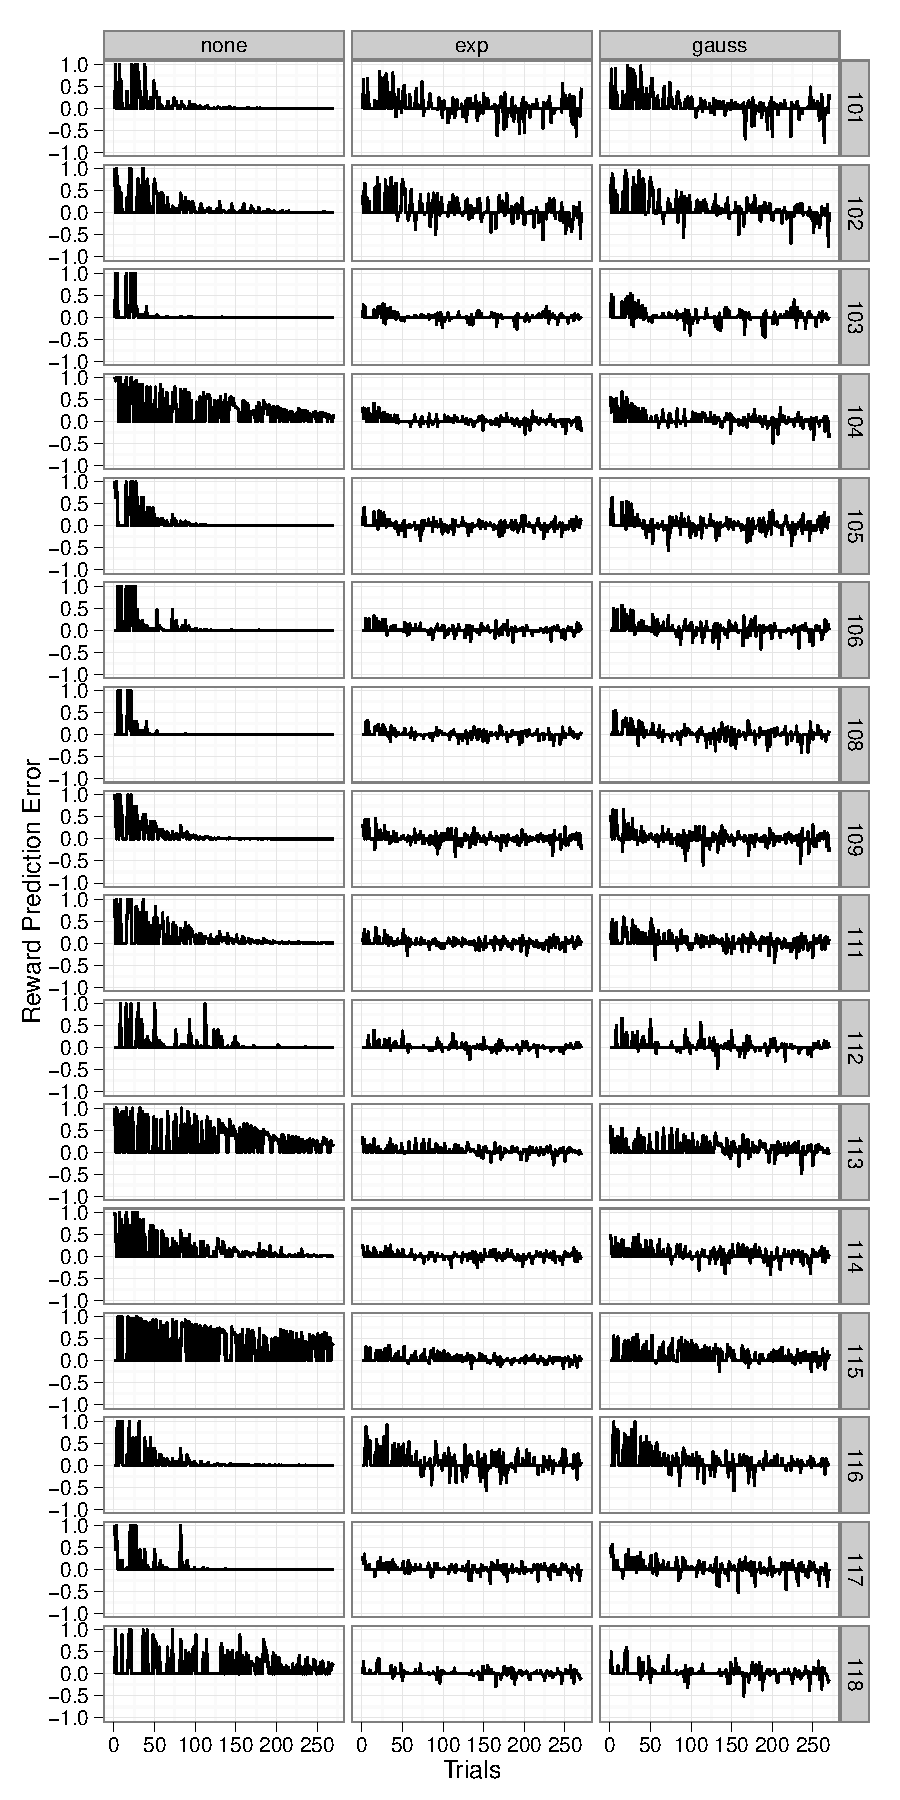
\includegraphics[width=0.6\textwidth]{f_rpe_acc}
    \centering
    \caption{Reward prediction errors for each of the three models plotted for each trial in the experiment, based on the $\{1,0\}$ coding scheme, which also represents the min-max range of the y-axis.  Each row is a single subject's data.  Each column matches one of the three models, classified by their similarity metric.}
    \label{fig:rpeacc}
\end{figure}
\begin{figure}[tp]
    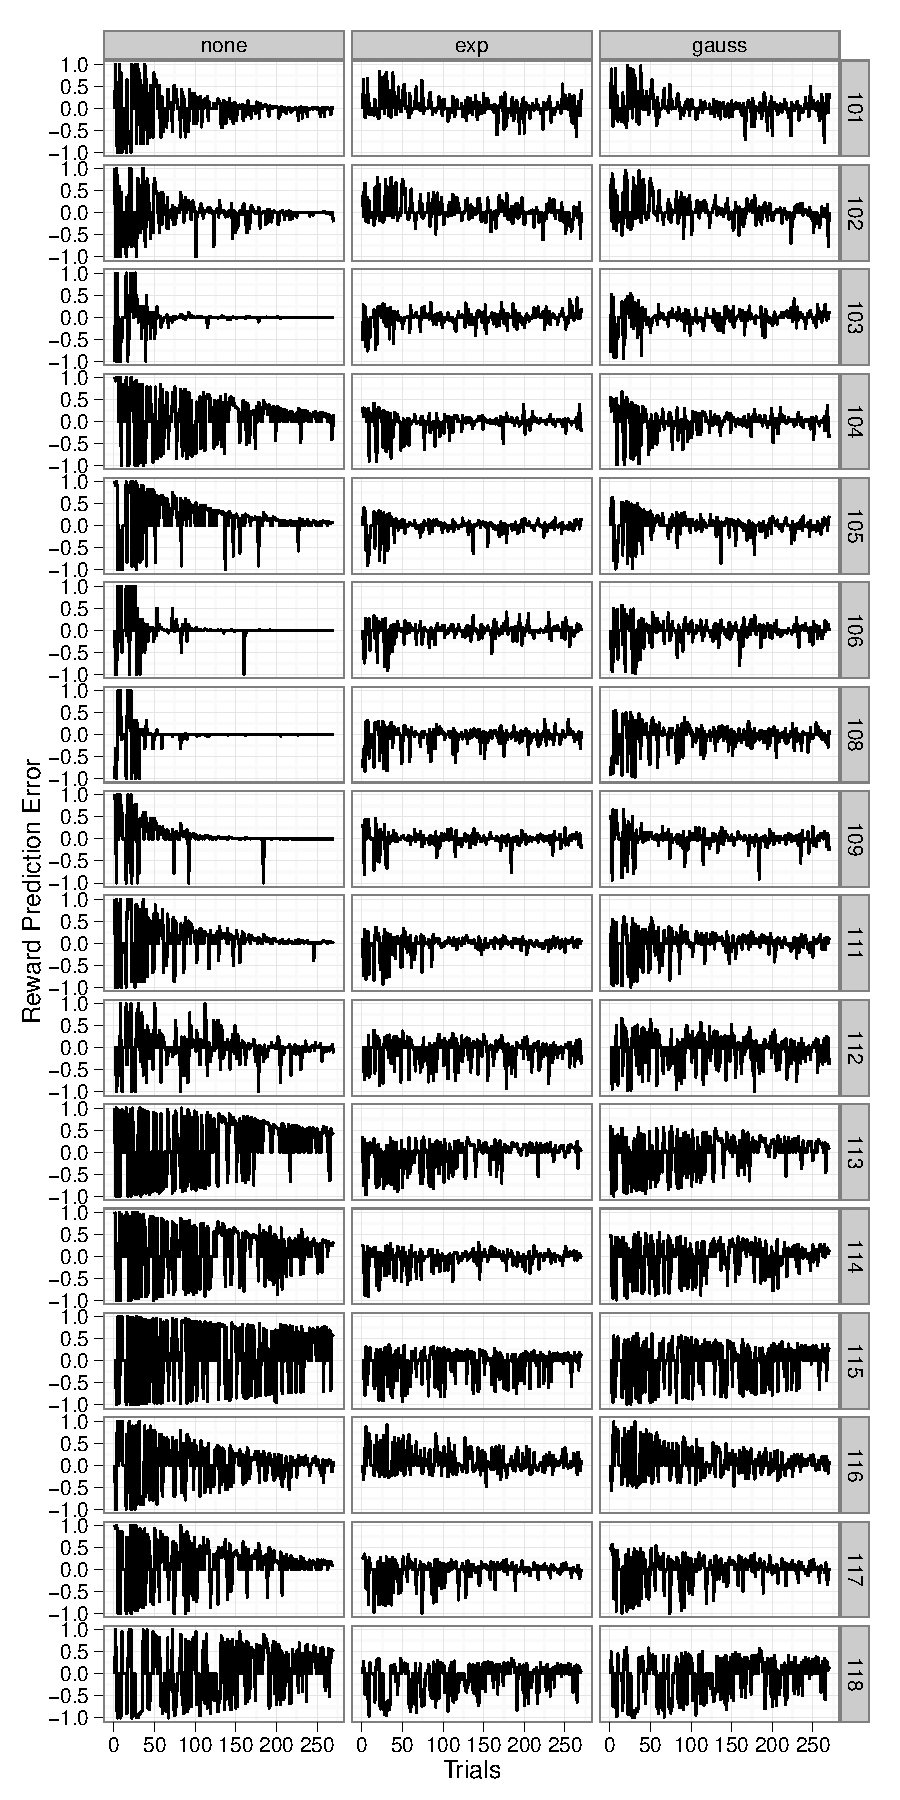
\includegraphics[width=0.6\textwidth]{f_rpe_gl}
    \centering
    \caption{Reward prediction errors for each of the three models plotted for each trial in the experiment, based on the $\{1,-1\}$ coding scheme, which also represents the min-max range of the y-axis.   Each row is a single subject's data.  Each column matches one of the three models, classified by their similarity metric.}
    \label{fig:rpegl}
\end{figure}

\begin{figure}[tp]
    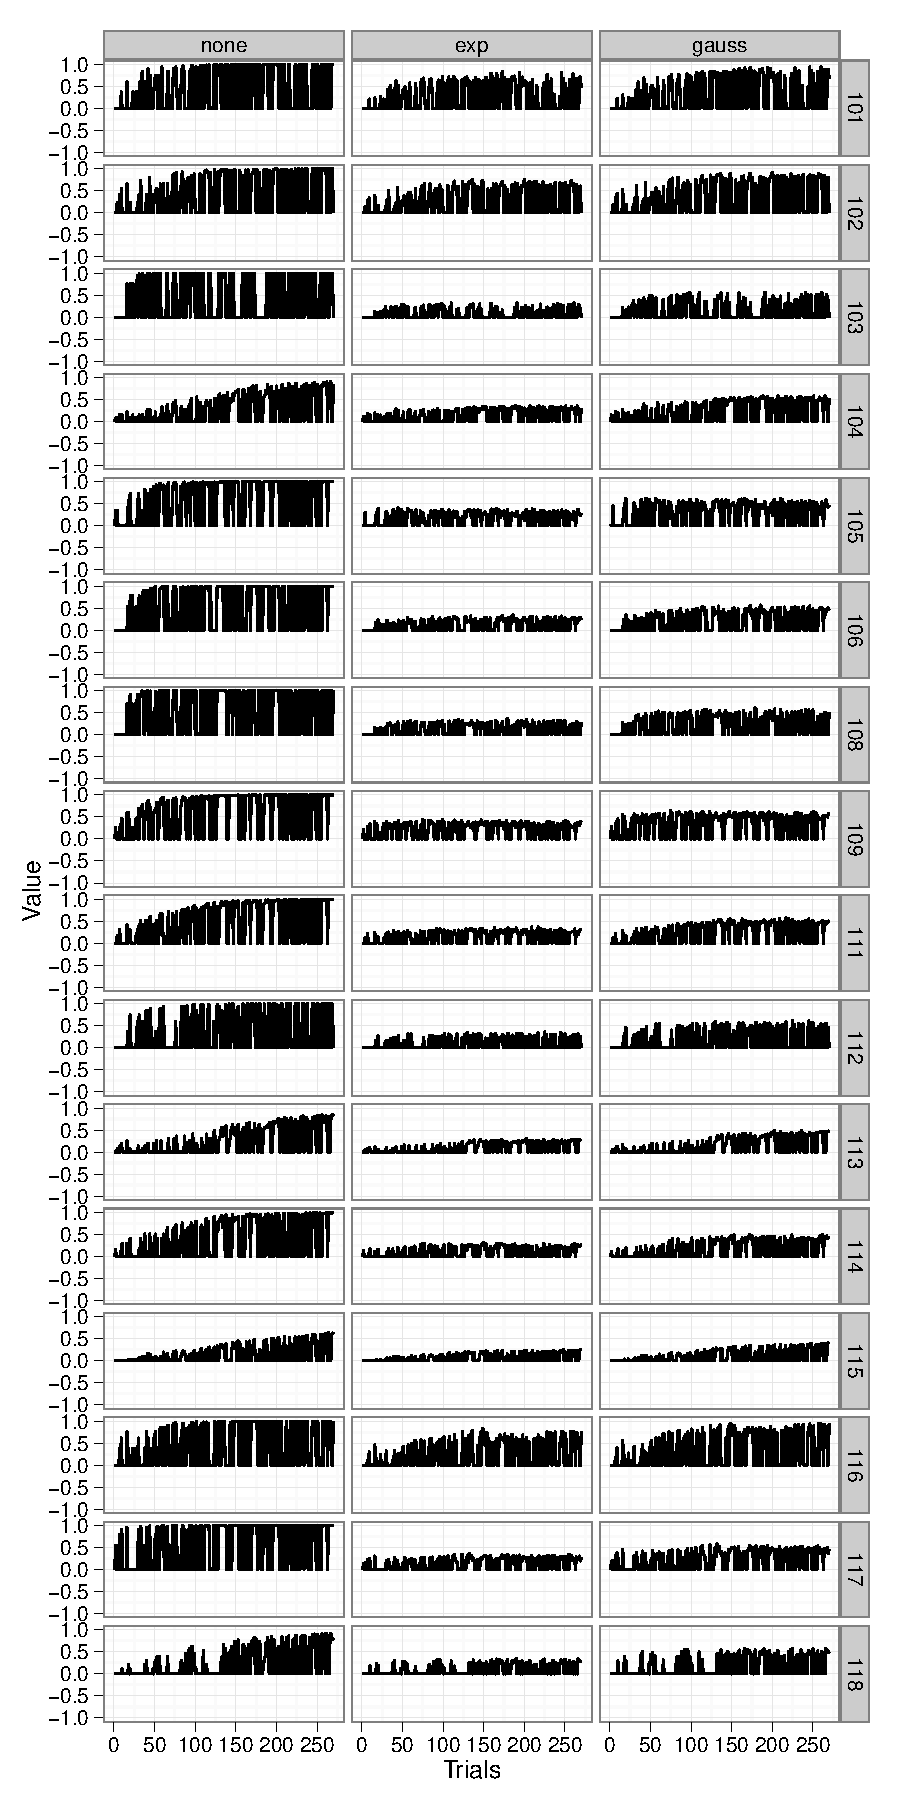
\includegraphics[width=0.6\textwidth]{f_value_acc}
    \centering    
    \caption{Value estimates for each of the three models plotted for each trial in the experiment, based on the $\{1,0\}$ coding scheme, which also represents the min-max range of the y-axis.  Each row is a single subject's data.  Each column matches one of the three models, classified by their similarity metric.}
    \label{fig:valueacc}
\end{figure}
\begin{figure}[tp]
    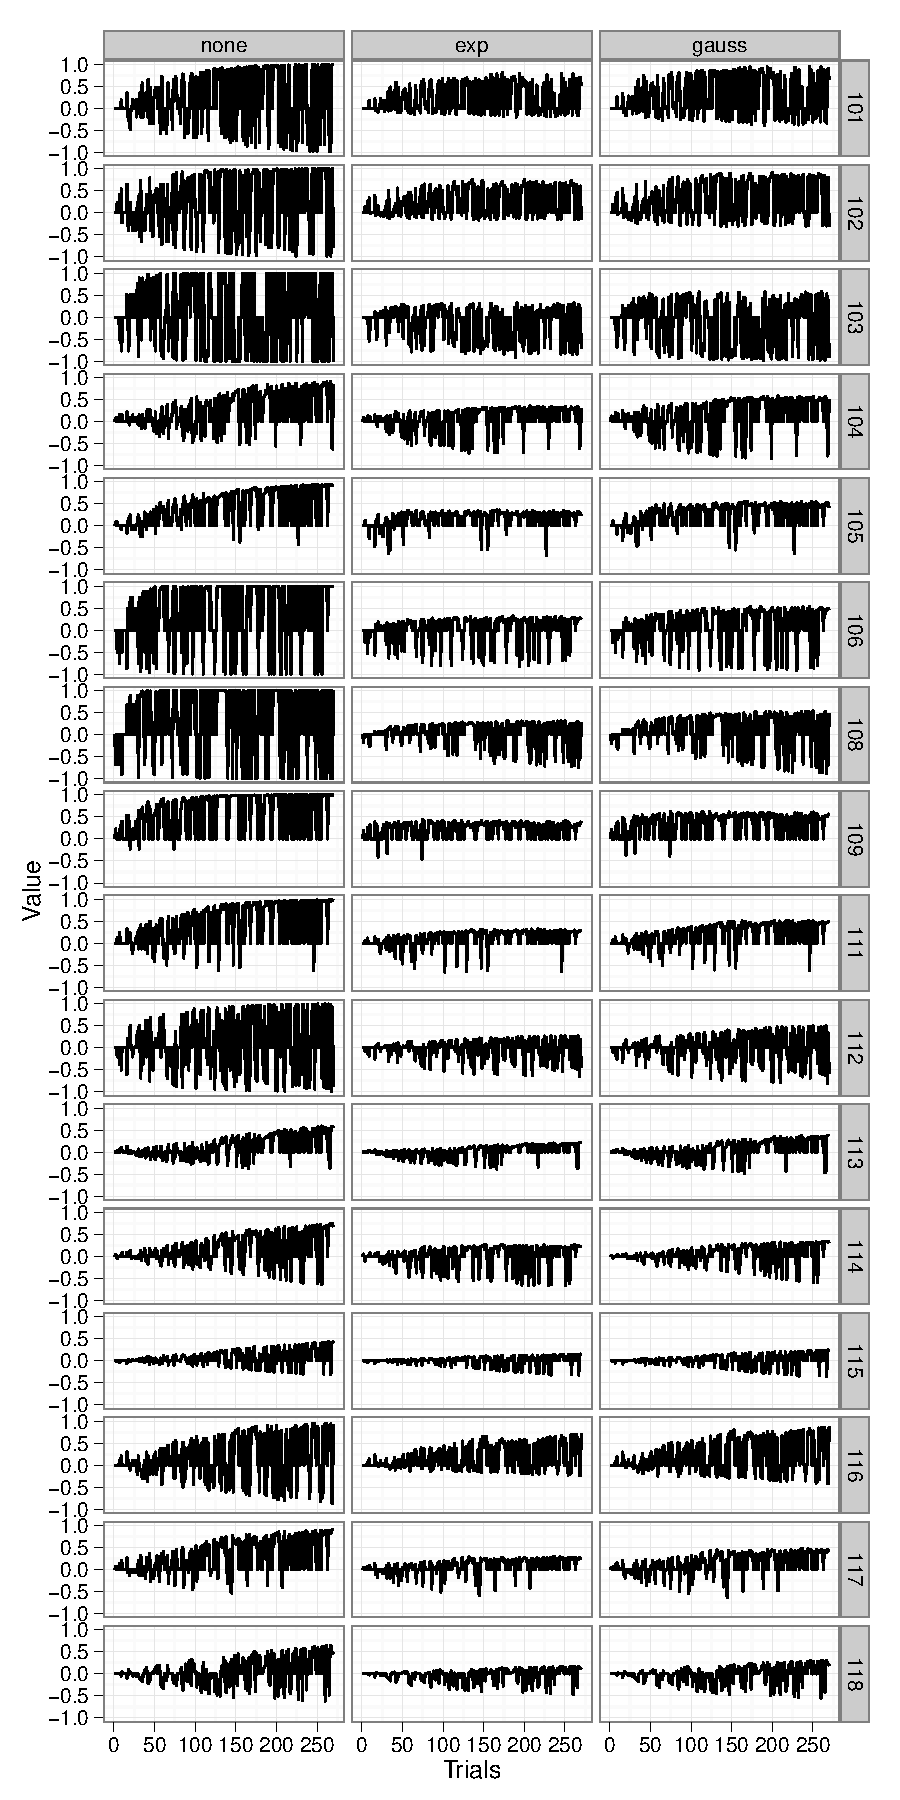
\includegraphics[width=0.6\textwidth]{f_value_gl}
    \centering
    \caption{Value estimates for each of the three models plotted for each trial in the experiment, based on the $\{1,-1\}$ coding scheme, which also represents the min-max range of the y-axis.   Each row is a single subject's data.  Each column matches one of the three models, classified by their similarity metric.}
    \label{fig:valuegl}
\end{figure}
\begin{figure}[tp]
    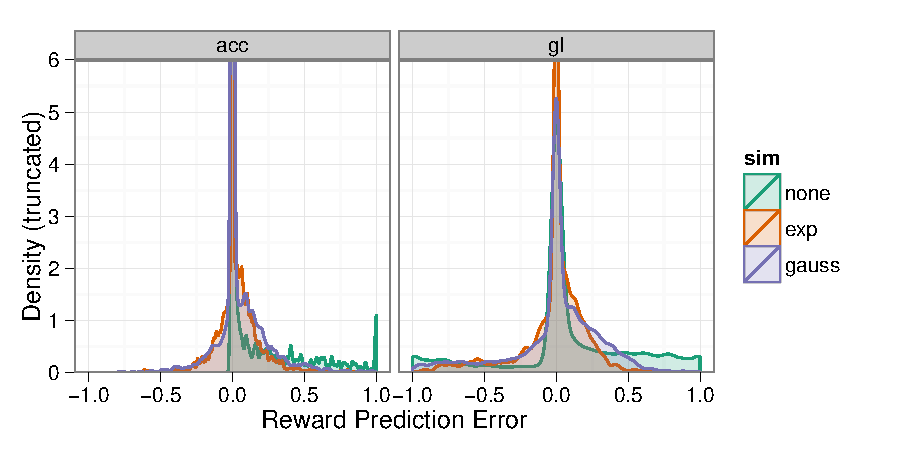
\includegraphics{f_density_rpe}
    \centering
    \caption{Density of reward prediction errors for all subjects.  The y axis is truncated at 6 to allow clear visualization of non-zero values.}
    \label{fig:denrpe}
\end{figure}

\begin{figure}[tp]
    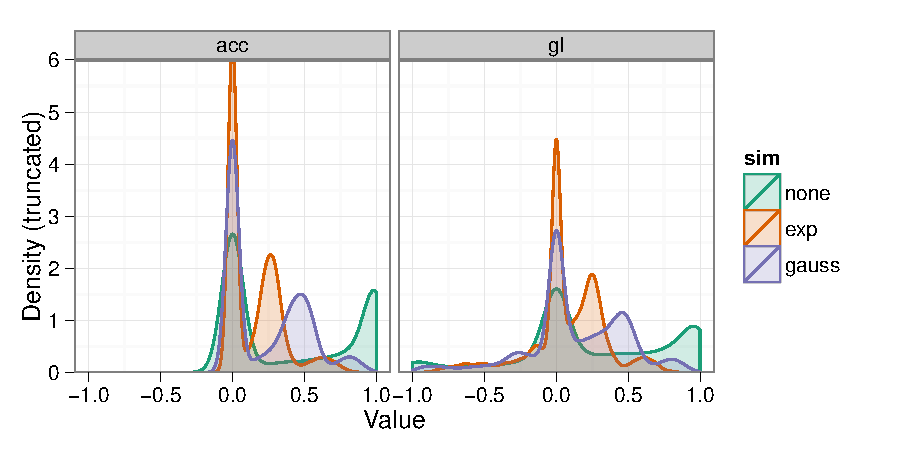
\includegraphics{f_density_value}
    \centering
    \caption{Density of value estimates for all subjects.  The y axis is truncated at 6 to allow clear visualization of non-zero values.}
    \label{fig:denvalue}
\end{figure}
\clearpage
  \section{Chapter 3 -- fMRI analyses} % (fold)
\label{sec:task_and_models}
This chapter has 4 parts, all address different aspects of fMRI data collection and analysis.  First is the methodolical details of the fMRI functional (i.e., BOLD) and structural acquisition, as well as the preprocessing of that data.  Little here exceeds or differs from current accepted fMRI data practices \cite{Poldrack:2008p6570,Amaro:2006p2638,Bullmore:1996p6538}.  Second null-hypothesis test thresholded maps of BOLD activity are considered (i.e. whole-brain patterns of activity are discussed).  The third section describes an alternative to the whole-brain analysis, focus on comparing BOLD time-courses from anatomical regions of interest to the reinforcement learning models from the previous chapter (p\pageref{sub:threemodels}).  In this, the focus is on ranking models using information theory metrics, not trying to select \emph{a} correct model as one might do in more traditional ROI analyses (for example, \citeA{Poldrack:2006p9841,Mars:2010p7999}).  Fourth is the results from the region of interest analyses described in part three.  These results are, in general, highly supportive of rewards as categories, though the argument for that conclusion is held off until the next, final, chapter (p\pageref{sec:dicussion}).

\subsection{An Acquisition}
\label{sub:acquired}
\subsubsection{Data details}
\label{subsub:datadetails}
fMRI data was acquired at the Intermountain Neuroimaging Consortium (INC) facility located at the University of Colorado at Boulder on a Siemens Allegra 3T (whole body) scanner.  All 18 right-handed participants were pre-screened for the typical fMRI exclusion factors (e.g., metal implants, mental disorders, etc).  High resolution anatomical data was acquired as a T1-weighted structural image, MPRAGE sequence, at 1x1x1 mm, (256 x 156 x 192) with a TR of 2530 ms, and TE of 1.64 ms, with a flip angle of 7$^\circ$.  All functional (i.e., BOLD) data was acquired with T2-weighted echo-planar imaging (EPI), at 2.29 x 2.29 x 4.00 mm (96 x 96 x 26), with a TR of 1500 ms, a TE a 25 ms, a flip angle of 75$^\circ$ and a FOV of 220 mm.

Four sets of functional data were acquired.  The first was of the ``refresher'' for part 1 of the behavioral training (p\pageref{subsub:whatwhen}), spanning 241 volumes.  The second and third spanned part 2 of the stimulus-responses learning task, divided into 2 (nearly) even sets lasting 390 and 394 volumes respectively (again see p\pageref{subsub:whatwhen}).  The fourth scan featured repeated presentation of gratings from both reward categories, in a random order.  The intent of this scan was to isolate rewarding activity outside the primary task. This localizer was not in the end useful (discussed on p\pageref{subsub:chunks}).

\subsubsection{Preprocessed (model) food}
\label{subsub:preprocessed}
Following DICOM to nifiti-1 conversion using dicom2nii (\url{http://www.mccauslandcenter.sc.edu/mricro/mricron/dcm2nii.html}), each dataset was subjected to the following preprocessing pipeline carried out in SPM8's batch mode (\url{http://www.fil.ion.ucl.ac.uk/spm/software/spm8/}).  For complete code see, \url{https://github.com/andsoandso/fmri/tree/master/catreward/spm\_m}.  Anatomical data was first segmented into white and grey matter regions \cite{Collignon:1995p9347}.  Based on these segments the parameters necessary for normalization into a standard reference space (T1 MNI-352, at 1 mm, MNI space or short) were calculated. Normalization had two steps.  The first was a Bayesian 12-parameter affine transformation \cite{Ashburner:1997p9348}.  The second was a set of nonlinear deformations, using a 1127 parameter discrete cosine transform \cite{Ashburner:1999p9350}.  Anatomical data was then resampled from 1.27 to 1.00 $mm^3$ using fourth degree $\beta$-splines, and finally, using the parameters above, normalized into MNI space.

To correct for the slight head movements that often occurring during scanning, movement regressors for all volumes of the functional data were first calculated \cite{Ashburner:1999p9350}.  No participant moved more than 1.5 mm, so all data was retained.  Functional data was then slice-time corrected, using slice 13 (the middle slice from the descending acquisition) as the reference, followed by coregisteration with the pre-processed (native-space) anatomical data, and resampling into 3 mm$^3$ voxels, again using fourth degree $\beta$-splines \cite{Collignon:1995p9347}.  Functional data was then normalized into MNI space using the anatomically-derived parameters above.  Finally, the functional data was spatially smoothed using a 6 mm FWHM Gaussian, though a copy of the unsmoothed data was retained for the ROI analyses (described on p\pageref{sub:regoins}).  Just prior to regression analysis, each voxel's time course was also low-pass filtered using finite impulse response model, with a cutoff at 0.008 Hz \cite{Kruggel:1999p9351}.  For all whole-brain analyses, the movement regressors were entered into the regression models as covariates, accounting for any head movement.  Given the large spatial averages employed in the ROI analyses these weren't motion corrected \cite{Poldrack:2007p8572}.

\subsubsection{The best of all possible signals}
\label{subsub:bestsignal}
In fMRI, and in general time-series analysis, there is an intrinsic trade-off between detecting a signal in the presence of noise and estimating the shape of that signal \cite{Dale:1999p7901,Birn:2002p1777,Liu:2004p2141}.   One way to optimize over both these conflicting objectives is to manipulate the trial order in a rapid event-related design \cite{Miezin:2000p7924}.  One state-of-the-art method for optimizing the trial ordering process is a genetic algorithm which uses two (weighted) loss functions, one for signal detection and one for time-course estimation \cite{Wager:2003p2980}. \citeA{Kao:2009p7899}, improved on Wager's (2003) initial design by adding in a loss function for psychological considerations, greatly improving execution speed and documentation.  As a result, Kao et al's (2009) method/code was used to optimize trial orders for part 1 and 2 of the behavioral task (p\pageref{subsub:whatwhen}), along with the reward category localizer scan (p\pageref{subsub:datadetails}).

\subsection{Mobs of Blobs}
\label{sub:blob}
All statistical parametric maps (below) were derived from a Random Effects analysis (RFX, or ``second-level'' in SPM8 jargon), multiple comparison corrected assuming Gaussian Random Fields using the Family Wise Error Rate (FWE) at the $p < 0.05$ level, with a minimum cluster size of 4 voxels \cite{Worsley:1996p9367}. 

Whole brain activity for the stimulus-response learning portion of the behavioral experiment (i.e., part 2, p\pageref{subsub:whatwhen}) was examined first by comparing all trials to the baseline (rest) condition.  This data is presented in two ways. First is the statistical thresholded image.  This contrast map showed significant bilateral activity in the cerebellum, insula and anterior cingulate ($t$(15) = 6.59, $p< 0.05$; Figure~\ref{fig:gl}).  Second is an overlay of the raw $t$-values, which allows for visual confirmation the observed significant effects were robust and widespread in their respective regions, but also allowed for the analysis of overall and sub-threshold patterns of activity.  These raw data suggested near threshold levels of activity in the head of the caudate, ventromedial, dorsolateral frontal cortices as well as (weaker) activity in the occipital lobe (Figure~\ref{fig:glraw}).  And indeed in a two-way ANOVA looking at that interaction between gains and losses, significant clusters were observed in head and body of caudate, insula, posterior and anterior cingulate with the posterior activation extending into the precuneus, as well as in dorsolateral (i.e middle frontal) PFC, and in ventrolateral PFC (Figure~\ref{fig:gxl}; $F$(1, 270) = 30.76, $p < 0.05$).  When gains and losses were examined separately, but again compared to rest, both had activity in the same areas as in the combined condition (not shown).

\begin{figure}[tp]
    \fitfigure{f_map_gl_p05}
    \centering
    \caption{Statistical parametric map for all trials in the stimulus-response learning task (i.e., part 2, p\pageref{subsub:whatwhen}), compared to the rest period.  \emph{Left} is a glass brain, showing all significant clusters.  \emph{Right} is a set of axial slices highlighting strong areas of activity overlaid onto the T1 MNI-352 template.  $Z$ is the height of the axial slice in MNI space.}
    \label{fig:gl}
\end{figure}

\begin{figure}[tp]
    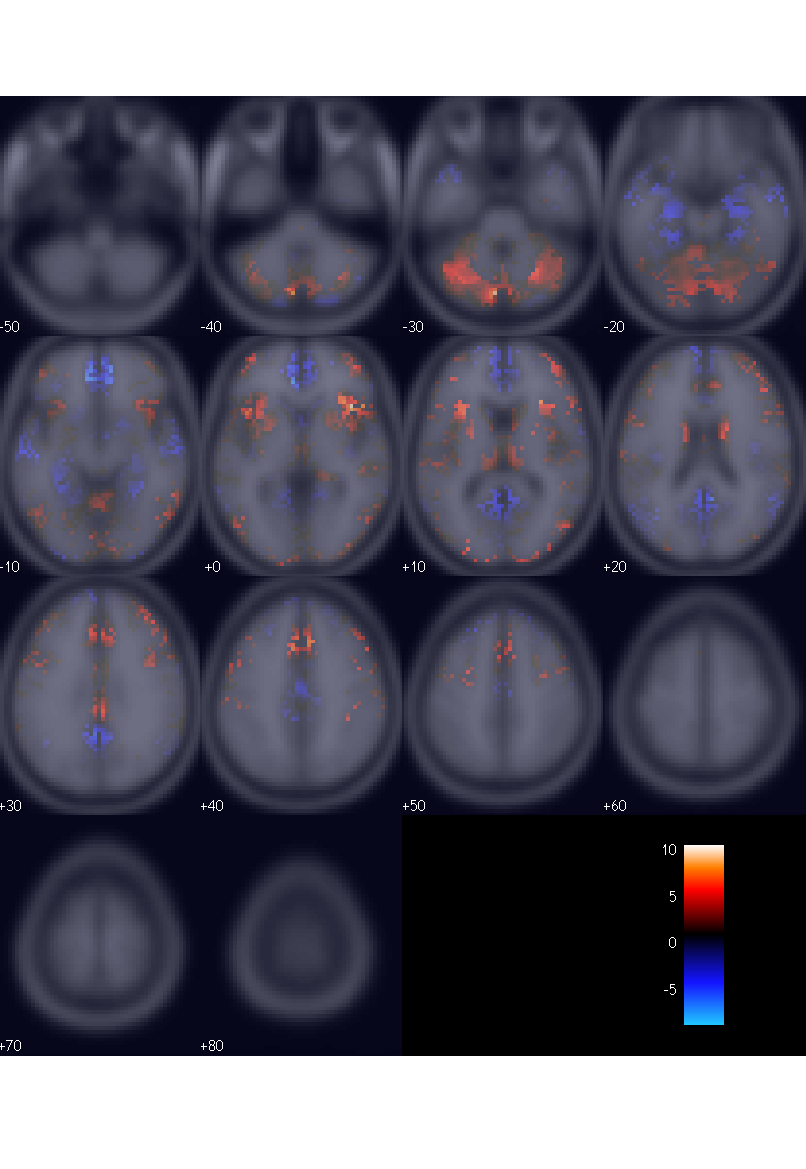
\includegraphics{f_map_gl_raw_t}
    \centering
    \caption{(The $t$-values for all trials in the stimulus-response learning task (i.e., part 2), compared to the rest period,  overlaid onto the T1 MNI-352 template.   Each number is the height of the axial slice in MNI space.}
    \label{fig:glraw}
\end{figure}

\begin{figure}[tp]
    \fitfigure{f_map_gxl_p05}
    \centering
    \caption{Statistical parametric map for all trials in the stimulus-response learning task (i.e., part 2) examining the interaction between gains and losses.  \emph{Left} is a glass brain, showing all significant clusters.  \emph{Right} is a set of axial slices highlighting strong areas of activity overlaid onto the T1 MNI-352 template.  $Z$ is the height of the axial slice in MNI space.}
    \label{fig:gxl}
\end{figure}

\subsection{Regions and Models}
\label{sub:regoins}
\subsubsection{The right chunks}
\label{subsub:chunks}
Following whole-brain analysis, regions of interest were selected using two separate yet related methods.  The first employed only regions from the Harvard-Oxford probabilistic anatomical atlas, using the 50\% cutoff \cite{Desikan:2006p9370}.  The second combined anatomical regions with functional clusters isolated using both the data collected during the second half of part 1 (i.e., the ``refresher'') and from the reward category localizer (p\pageref{subsub:datadetails}).  Comparisons between them showed the anatomically-limited functional clusters and the entire anatomical regions displayed very similar results.  So to limit the complexity of later analyses, and to increase power, functional clusters were discarded in favor of the larger anatomical regions.  Most anatomical regions of interest were selected \emph{a priori} based on previous studies of reinforcement and category learning (see the \emph{Introduction} for a review).  Left and right subcortical regions of interest were the dorsal caudate, ventral striatum/nucleus accumbens, and putamen.   Bilateral cortical areas were the middle frontal cortex (i.e., dorsolateral PFC), frontal medial cortex (which contains ventrolateral PFC), and orbital frontal cortex.  Based on the whole-brain maps (p\pageref{sub:blob}), regions for the insula, anterior and posterior cingulate (ACC and PCC for short) were included as well. While these is no strong \emph{a priori} hypothesis for the role of these regions may play or may not play, activity in each of these \emph{post hoc} regions is common to human category learning experiments \cite{LopezPaniagua:2011p8296,Seger:2010p7188,Cincotta:2007p6672,Seger:2006p5447,Seger:2005pd}.


% -- PROOFED ABOVE
\subsubsection{A way to(o) many}
\label{subsub:tomany}
There are 6 models under evaluation: the three kinds of similarity adjustment (``none'', ``exp'', and ``gauss'') multiplied by the two possible reward codes (``acc'' and ``gl''), with the two terms of interest (i.e., value and the reward prediction error), that is 12 comparisons.  The were also a number of \emph{a priori} confounds to our signals of interest including the similarity metrics, the reward codes, and the grating parameters, bringing the total to 23.  As the models are not nested\footnote{
    Often defined by whether or not two models can be made identical by adding or subtracting parameters \cite{Forster:2000p9623}} and therefore not amenable to $F$-tests -- the common statistical way to compare model fits -- an alternative approach was called for.  Further complicating the issue was the fact that each of the models is covariate, if not collinear, with the others.  To top it off, none of the three similarity-adjustments are statistically independent; reinforcement learning can be viewed as a regression of the reward code onto behavioral choices.  All these factors combined would make statistical testing difficult, to say the least.  But fortunately finding \emph{the} best model is not the goal.  

The latest recordings of phasic (i.e., reward prediction) activity in the VTA/SNc suggests a complicated reward and prediction error coding scheme (see p\pageref{subsub:expectations}), wherein several separate sets of calculations may be carried out independently \cite{Kim:2006p1063, Matsumoto:2009p7219, Smith:2011p8133}.  The observed BOLD signal is then an aggregate of these many activities. It is possible, even likely, then that more than one of the models is correct making null hypothesis tests an incorrect choice.  Model selection is the right choice.

Model selection is the process of finding a \emph{family} of models that best predict a given dataset \cite{Rao:2001p9457}.  Most techniques try to wisely balance parsimony with increasing fit (i.e., solving the bias versus variance dilemma \cite{Geman:1p9469}).  Unfortunately most model selection techniques require assumptions the models cannot meet (e.g., statistical independence).  The few that can tend to be complex recent statistical inventions.  Rather than navigate those troubled and unproven waters, a simpler approach was taken. Each model was independently examined and ranked, in an approach loosely similar to model averaging \cite{Forster:2000p9623}.

An AIC score (Akaike Information Criterion \cite{Akaike:1974p9530}) was assigned to each of the models/codes for every participant and region of interest.  The absolute AIC score across participants is not however meaningful.  Only the relative values are of interest \cite{Wagenmakers:2004p9472}.  As a result, individual's scores were normalized and ranked by subtracting the best (lowest) score from each \cite{Anderson:2000p9475}. The normalized set was then transformed to Akaike Weights, a way to easily compare the conditional probabilities of each model being true \cite{Wagenmakers:2004p9472}.  The Akaike Weights were then averaged across participants for each model and region of interest.

\subsubsection{Information on information}
\label{subsub:way}
AIC is a measure of loss; how much information is lost by substituting the model for the true distribution, i.e., the data.  The lower the AIC score, the better the model.  Unlike null hypothesis tests and Bayesian measures, AIC-based methods do not seek to find \emph{a} truth, but instead serve to rank models.  AIC offers then only relative insight, and is unable to make any claims about absolute significance.  Significance is a separate question, one to be returned to later.  Besides this limitation, AIC has some substantial advantages. Five are reviewed below.

One, unlike maximum-likelihood, AIC is designed to be a parsimonious score.  It penalizes for additional parameters.  It may therefore choose a worse model (as measured by likelihood or mean squared error) over a better but more complex one. This is the essence of Occam's razor\footnote{Famously and pithily expressed as, ``Entities are not to be multiplied beyond necessity''.}. 

Two, it fits with the process of science.  When designing an experiment it is rare that there are only two possible outcomes, instead typically there are several competing hypothesis, some of which may not be mutually exclusive.  AIC's focus on relative differences and evidential weights meshes perfectly with the reality of multiple working hypotheses \cite{Burnham:2004p9621}.

Three, truth can remain elusive.  A common alternative to AIC is BIC, the Bayesian Information Criterion.  Like AIC, BIC is derived from the log-likelihood of a model, however its derivation requires a rather strict (and often unrealistic) assumption -- that the true model is among the candidates \cite{Forster:2000p9623}.  And while it may be philosophically debatable whether any mathematical model can \emph{completely} describe reality, in this study the models are incomplete.  As, one, the human reinforcement learning literature contains several recent theoretically unaccounted for findings and, two, there are theoretical developments not include here to keep the models tractable (see the \emph{Introduction} for a review).  

Four, AIC values are easily interpretable once they're transformed to Akaike Likelihoods or Weights\footnote{
    Likelihood for model $k$ among $K$ working hypotheses/models is given by $L_k = e^{-0.5({AIC}_k - {min}_{K}{(AIC)})}$, which is then normalized, becoming an Akaike Weight by $w_k = L_k / \sum\limits_{k=1}^K L_k$ \cite{Burnham:2004p9621}.}.  The likelihood is, as you would expect, simply the likelihood the model is correct (based on the information loss associated with it), while the Akaike Weights are normalized likelihoods.  As the Weights sum to one, the conditional likelihood of one model compared to another is just the ratio of their weights \cite{Burnham:2004p9621}.  For example, the conditional likelihood of model A over model B is just $w_A/w_B$.  That is, the likelihoods and Akaike Weights are intrinsically measures of effect size \cite{Anderson:2000p9475,Forster:2000p9623}.  Despite the fact that it is often used to express the likelihood of correctly rejecting the null hypothesis, the $p$ value is not a measure of effect, as $p$ is contingent not just on effect size but on sample number.  
    
    Five, AIC has a history with models of categorization. \citeA{McKinley:1996p9532,Maddox:2001p9533}, among several others, used AIC to compare behavioral results to several alternative models of categorization.
    
\subsubsection{F-them}
\label{subsub:F}
AIC ranks offer no information about significance, in the familiar null hypothesis sense, or about the absolute fit of the model.  Both of these were addressed in a series of $F$-tests run prior to AIC analysis.  These (fixed-effect, across participant) omnibus tests asked whether the total set of regression parameters for each linear model (described below) could explain the BOLD time series better than chance (i.e could the null hypothesis (of 0) be rejected).  Keeping with recommendations of \citeA{Burnham:2004p9621, Forster:2000p9623}, who argue that as AIC and significance tests are so dissimilar that direct comparison/interaction between them will be at best misleading, the models are not discarded based on significance.  All models are retained, and later AIC ranked.  The $F$-tests are a separate measure whose results are integrated during interpretation, not during model selection.

\subsubsection{Code, BOLD, and models.}
\label{sub:cmb}
A total of 23 models were compared for each of the 12 regions of interest for each of the 16 subjects, 4416 comparisons in total.  Each of the models is described below (Table 1).  In general, a time-series (e.g the reward prediction error for each trial or the similarity for that trial's outcome) was convolved with a ``canonical''  haemodynamic response function, a mixture of gamma functions that serves as a parsimonious estimate of the (instantaneous) BOLD response \cite{Friston:1998p2022}.  The convolved series was then low-pass filtered, matching the treatment of the BOLD data (p\pageref{subsub:preprocessed}).  Each convolved and filtered model was then regressed onto the BOLD response for each participant's region of interest, retaining all parameters and fit measures inside subject-level HDF5 files.  The HDF5 format offers high performance read/write operations, and widespread support across several scientific programming languages (\url{http://www.hdfgroup.org/HDF5/}).

No available fMRI analysis package returns AIC scores (or measures that could be converted to such) and none allow for the efficient (i.e programmatic) analysis of many competing computational models. So a region of interest focused fMRI analysis tool was created in Python (v2.7.1) to meet those two needs.  This module, simply named ``roi'', has since been release under the BSD license and is available for download at \url{https://github.com/andsoandso/roi}. It relies on the nibabel library to read the nifiti-1 files  (v1.2.0; \url{http://nipy.org/nibabel}), nitime for time-series analysis, (v0.4; \url{http://nipy.sourceforge.net/nitime/}) Numpy for generic numerical work (v1.6.1; \url{http://numpy.scipy.org/}), with the GLS function from the scikits.statsmodels module handling the regressions (v0.40; \url{http://statsmodels.sourceforge.net/}).  Model-to-BOLD fit parameters, as well as other useful metadata, was then extracted and stored in text files suitable for importing into R (v2.15.1; \url{http://www.r-project.org/}).  All plotting and model ranking (as well as the $F$-tests) were carried out in R.  For complete BSD licensed code see, \url{https://github.com/andsoandso/fmri/tree/master/catreward/roi/results}.

\subsubsection{Our kinds of models}
\label{subsub:ourkinds}
To ease visualization and analysis each of the models was classified into one of 5 families.  Family one, denoted ``boxcar'', was identical to that first used in the whole-brain analysis (p\pageref{sub:blob}) -- all trials versus the rest condition.  This is a univariate time-series that predicts no trial-specific effects; No matter the task the brain, thus the BOLD response, just flicks on then off.  It serves as a useful standard against which to compare the model-based regressors.  The next two families were controls (i.e., \emph{a priori} covariates). The reward codes, both raw and similarity adjusted, were in one family (``control\_reward'') and in the other were the similarity metrics and grating parameters (``control\_similarity'').  The fourth family contained all the reward prediction errors (``rpe'').  The fifth contained all value estimates (``value'').

\newpage
\begin{center}
    \begin{longtable}{ | l | l | l | p{6cm} |}
    \caption{All models, their designations (Codes), families, and descriptions.}\\
    \hline
    Number & Code & Family & Description \\ \hline
         1 & 0\_1 & boxcar & The simplest model, a univariate analysis of all conditions. \\ \hline
         2 & acc & control\_reward & Behavioral accuracy. \\ \hline
         3 & acc\_exp & control\_reward & Behavioral accuracy, diminished by (exponential) similarity. \\ \hline
         4 & acc\_gauss & control\_reward & Behavioral accuracy, diminished by (Gaussian) similarity. \\ \hline
         5 & gl & control\_reward & Gains and losses. \\ \hline 
         6 & gl\_exp & control\_reward & Gains and losses, diminished by (exponential) similarity. \\ \hline
         7 & gl\_gauss & control\_reward & Gains and losses, diminished by (Gaussian) similarity. \\ \hline
         8 & rpe\_acc & rpe & Reward prediction error - derived from accuracy. \\ \hline
         9 & rpe\_acc\_exp & rpe & Reward prediction error - derived from accuracy diminished by (exponential) similarity. \\ \hline
        10 & rpe\_acc\_gauss & rpe & Reward prediction error - derived from accuracy diminished by (Gaussian) similarity. \\ \hline
        11 & value\_acc & value & Value - derived from accuracy. \\ \hline
        12 & value\_acc\_exp & value & Value - derived from accuracy diminished by (exponential) similarity. \\ \hline
        13 & value\_acc\_gauss & value & Value - derived from accuracy diminished by (Gaussian) similarity. \\ \hline
        14 & rpe\_gl & rpe & Reward prediction error - derived from gains and loses. \\ \hline
        15 & rpe\_gl\_exp & rpe & Reward prediction error - derived from gains and losses diminished by (exponential) similarity. \\ \hline
        16 & rpe\_gl\_gauss & rpe & Reward prediction error - derived from gains and losses diminished by (Gaussian) similarity. \\ \hline
        17 & value\_gl & value & Value - derived from gains and losses. \\ \hline
        18 & value\_gl\_exp & value & Value - derived from gains and losses diminished by (exponential) similarity. \\ \hline
        19 & value\_gl\_gauss & value & Value - derived from gains and losses diminished by (Gaussian) similarity. \\ \hline 
        20 & exp & control\_similarity & Outcome similarity (exponential). \\ \hline
        21 & gauss & control\_similarity & Outcome similarity (Gaussian). \\ \hline
        22 & angle & control\_similarity & Grating angle parameter. \\ \hline
        23 &width & control\_similarity & Grating width parameter. \\ \hline
    \end{longtable}
\end{center}


\subsection{Model Results}
\label{sub:modelresults}
The many results are dicussed, first by subcortical areas then moving on to the cortical.  The general analysis strategy was to first find the top family, indicated by the largest family-average Akaike Weight.  Then the next highest scoring to family was examined to see if it was close to the top (i.e., $\le$1.5 times as likely).  If it was both, families were included.   The next step examined the relative likelihood of each model in the top family/families.  Within-family models that were about $\ge$1.5 times more likely then their neighbor were dubbed ``substantively more informative''.  Like the significance thresholded in null hypothesis tests this $\ge$1.5 is an arbitrary threshold.  However in order discuss and interpret these results a line must be drawn between meaningful and not, and $\ge$1.5 is a good minimum cutoff \cite{Anderson:2000p9475, Forster:2000p9623}.  As was stated at the outset, more than one model may be right.  Thus the threshold was treated as a loose cutoff.  To get a sense of overall model quality, I the likelihood of the best model over the boxcar (i.e., the non-parametric standard) was calculated.  Finally all models, not just the top family, were assesed for any outliers that may have scored well despite their families overall poor performance.

As this was the first attempt to AIC-rank models of fMRI data, and while much thought and research was put into the above scheme, it may be flawed.  It is also arbitrary (beyond the $\ge$1.5 cutoff); Why not discuss the top 3, or 4 families, or even just include them all?  To attempt then to minimize the effect of these arbitrary, but necessary, decisions the complete set of models (and $F$-tests) are included for every region of interest.


\subsubsection{From up high}
\label{subsub:fromuphigh}
For eight of the twelve regions of interest the ``rpe'' family scored highest.  Of these eight, five were best described by ``rpe\_acc\_gauss''.  The next best family was ``control\_similarity'' with 3 regions, followed by ``boxcar'' with 1.  Notably, ``value'' was not the most informative model family for any region of interest, and indeed the one region (ACC) for which it was second, ``rpe'' was 1.8 times more likely.


\subsubsection{Under cortical}
\label{subsub:belowctx}
In the dorsal caudate (Figure~\ref{fig:caudate}), only the ``rpe'' family offered a more informative fit that the ``boxcar'', being 2.61 times more likely in the left and 2.85 in the right (abbreviated as left/right: 2.61/2.85 from here on).  Bilaterally, and using the ``acc'' coding scheme, the Gaussian similarity-adjusted model (i.e., ''rpe\_acc\_gauss'') was substantively more informative than either unadjusted model (``rpe\_acc'' -- 1.45/1.54 or ``rpe\_gl'' 1.82/1.70).  Surprisingly, given its similarity to the Gaussian adjustment, ``rpe\_acc\_exp'' scored no better than the unadjusted models (above).  In what will become a reoccurring theme when examining the $F$-tests, all models were significant bilaterally in the dorsal caudate (Figure~\ref{fig:fvalcaudate}).  And while the $F$-values themselves to some degree mimic the patterns of the Akaike Weights, it would not be possible to reliably disassociate them given the slight relative differences.  

Compared to the ``boxcar'', the putamen was also best described by the ``rpe'' family (1.53/2.31).  However compared to caudate the putamen displayed markedly different within-family activity (Figure~\ref{fig:caudate} compared to~\ref{fig:putamen}). The ``rpe\_acc'' model was more substantively more likely (1.67/1.66) than the next highest ranking similarity model (i.e., ``rpe\_acc\_gauss'').  However due to the marginal bilateral significance (Figure~\ref{fig:fvalputamen}), this interesting reversal must be viewed cautiously.  The bilateral consistency in the Akaike Weights does offer some room for optimism (Figure~\ref{fig:putamen}, specifically refering to the consistency and relative strength of ``rpe\_acc'').

The right and left halves of the nucleus accumbens, the ventral portion of the striatum, were quite divergent in their fits (Figure~\ref{fig:accumbens}).  However both ranked the ``control\_similarity'' family as the most informative, however this family was only about 1.10 times more likely than the next family (``rpe''), which itself was not substantively better then its neighbor, and so on.  So while there is strong evidence that the top models, ``angle'' in left (3.07) and ``rpe\_gl'' (3.06) in the right, are better than ``boxcar'', the overall bilateral heterogeneity, weak family effects, combined with by-and-large non-significant outcomes on the left half, and weak $F$-values on the right (Figure~\ref{fig:fvalaccumbens}), suggest this region was not strongly activated by the task.  Further analysis is therefore futile.

\begin{figure}[tp]
    \fitfigure{f_meanbar_run4_c_aic_w_bilat_Caudate}
    \centering
    \caption{Dorsal caudate (left and right) -- Akaike Weights for all models.  Colors indicate model family (see p\pageref{sub:cmb} for details). Bars represent standard errors.}
    \label{fig:caudate}
\end{figure}
\begin{figure}[tp]
    \fitfigure{f_plot_run4_c_fvalue_bilat_Caudate}
    \centering
    \caption{Dorsal caudate (left and right) -- $F$-values for all models.  Significance-level is denoted by the saturation, where the $p <$ 0.05 level is significant, and trend is between $p <$ 0.05 and 0.10.  Colors indicate model family (see p\pageref{sub:cmb} for details).}
    \label{fig:fvalcaudate}
\end{figure}

\begin{figure}[tp]
    \fitfigure{f_meanbar_run4_c_aic_w_bilat_Putamen}
    \centering
    \caption{Putamen (left and right) -- Akaike Weights for all models.  Colors indicate model family (see p\pageref{sub:cmb} for details). Bars represent standard errors.}
    \label{fig:putamen}
\end{figure}
\begin{figure}[tp]
    \fitfigure{f_plot_run4_c_fvalue_bilat_Putamen}
    \centering
    \caption{Putamen (left and right) -- $F$-values for all models.
    Significance-level is denoted by the saturation, where the $p <$ 0.05 level is
    significant, and trend is between $p <$ 0.05 and 0.10.  Colors indicate model family (see p\pageref{sub:cmb} for details).}
    \label{fig:fvalputamen}
\end{figure}


\begin{figure}[tp]
    \fitfigure{f_meanbar_run4_c_aic_w_bilat_Accumbens}
    \centering
    \caption{Nucleus Accumbens (left and right) -- Akaike Weights for all models.  Colors indicate model family (see p\pageref{sub:cmb} for details). Bars represent standard errors.}
    \label{fig:accumbens}
\end{figure}
\begin{figure}[tp]
    \fitfigure{f_plot_run4_c_fvalue_bilat_Accumbens}
    \centering
    \caption{Nucleus accumbens (left and right) -- $F$-values for all models.
    Significance-level is denoted by the saturation, where the $p <$ 0.05 level is
    significant, and trend is between $p <$ 0.05 and 0.10.  Colors indicate model family (see p\pageref{sub:cmb} for details).}
    \label{fig:fvalaccumbens}
\end{figure}

\subsubsection{On that thinking sheet}
\label{subsub:onsheet}
The insula was the one region, both cortically and subcortically, to be nearly equally well described both by the ``acc'' and ``gl'' reward codes (Figure~\ref{fig:insula}).  In the top ranking ``rpe'' family (which was 1.37 times more likely than its neighbor ``control\_similarity'', and 2.31 more likely than the ``boxcar'') within-family models showed divergent patterns based on the code.  The ``acc'', ``rpe\_acc'' and ``rpe\_acc\_gauss'' models dominated ``rpe\_acc\_exp'' (around 1.4).  The ``gl'' code had the opposite effect, ``rpe\_gl\_exp'' dominated ``rpe\_gl'' and ``rpe\_gl\_gauss'' by a somewhat similar amount (1.20).  The strong overall significance of all models (Figure~\ref{fig:fvalinsula}) suggests these relative rankings may reflect truth; like the dorsal caudate the $F$-values the have same patterns as Akaike Weights.

Both the ACC and PCC displayed very similar rankings of their Akaike Weights (compare Figures~\ref{fig:ant} to~\ref{fig:post}), so they'll be discussed as one.  Again the ``rpe'' family dominated (respectively 2.07 and 1.77 times more likely compared to the nearest neighbor, 2.86 and 2.88 times more likely then the ``boxcar'').  Unlike the caudate and insula, the 2 similarity-adjustment models (``rpe\_acc\_gauss'' and ``rpe\_acc\_exp'') were consistently more informative than the reward unadjusted (``rpe\_acc'').  Looking at the $F$-tests, both regions, especially in the ``rpe'' family were, were reasonably significant (Figure~\ref{fig:fvalant} and~\ref{fig:fvalpost}).

Like the orbital frontal (below), ``boxcar'' was the most informative family for the middle frontal cortex (Figure~\ref{fig:dlpfc}), however model-wise ``rpe\_acc'' was 2.07 times more likely.  The strong $F$-values for all models, and ``rpe\_acc'' especially (the largest observed for all models and regions; Figure~\ref{fig:fvaldlpfc}), lend strong support then for selecting ``rpe\_acc'' as the sole best explanation of this regions activity.

Both the frontal medial (ventrolateral) and orbital frontal results are difficult to interpret, but for different reasons.  Nearly all families, and models, in the in frontal medial cortex ranked as substantively more likely that the ``boxcar'' (ranging, at the family level, from 2.13 for ``control\_similarity'' to 1.75 for ``value'', with higher scores for individual models).  However none of the models were substantively (or even slightly) more likely than any of their neighbors.  So while, as measured by the $F$-tests, there was significant activity in medial frontal (Figure~\ref{fig:fvalvmpfc}) it is not well accounted for by any of the candidate models.  Orbital frontal cortex though has the opposite problem.  The ``boxcar'' had the largest Akaike Weight (Figure~\ref{fig:ofc}).  However at the model-level ``rpe\_acc\_gauss'' and ``rpe\_acc'' both score slightly better (1.32 and 1.34, respectively).  However these slight increase are weak evidence when the alternative is that nothing has changed from trial-to-trial (i.e., the ``boxcar'' model).  Additionally as ACC and OFC are tightly functionally interconnected \cite{Rudebeck:2008p4712}, these weak likelihoods may be carryover from the strong ``rpe'' signals observed in the ACC (Figure~\ref{fig:ant}).

\begin{figure}[tp]
    \fitfigure{f_meanbar_run4_c_aic_w_Insular_Cortex}
    \centering
    \caption{Insula -- Akaike Weights for all models.  Colors indicate model family (see p\pageref{sub:cmb} for details). Bars represent standard errors.}
    \label{fig:insula}
\end{figure}
\begin{figure}[tp]
    \fitfigure{f_plot_run4_c_fvalue_Insular_Cortex}
    \centering
    \caption{Insula -- $F$-values for all models.
    Significance-level is denoted by the saturation, where the $p <$ 0.05 level is
    significant, and trend is between $p <$ 0.05 and 0.10.  Colors indicate model family (see p\pageref{sub:cmb} for details).}
    \label{fig:fvalinsula}
\end{figure}


\begin{figure}[tp]
    \fitfigure{f_meanbar_run4_c_aic_w_Cingulate_Gyrus_anterior_division}
    \centering
    \caption{ACC -- Akaike Weights for all models.  Colors indicate model family (see p\pageref{sub:cmb} for details). Bars represent standard errors.}
    \label{fig:ant}
\end{figure}
\begin{figure}[tp]
    \fitfigure{f_plot_run4_c_fvalue_Cingulate_Gyrus_anterior_division}
    \centering
    \caption{ACC -- $F$-values for all models.
    Significance-level is denoted by the saturation, where the $p <$ 0.05 level is
    significant, and trend is between $p <$ 0.05 and 0.10.  Colors indicate model family (see p\pageref{sub:cmb} for details).}
    \label{fig:fvalant}
\end{figure}


\begin{figure}[tp]
    \fitfigure{f_meanbar_run4_c_aic_w_Cingulate_Gyrus_posterior_division}
    \centering
    \caption{PCC -- Akaike Weights for all models.  Colors indicate model family (see p\pageref{sub:cmb} for details). Bars represent standard errors.}
    \label{fig:post}
\end{figure}
\begin{figure}[tp]
    \fitfigure{f_plot_run4_c_fvalue_Cingulate_Gyrus_posterior_division}
    \centering
    \caption{PCC -- $F$-values for all models.
    Significance-level is denoted by the saturation, where the $p <$ 0.05 level is
    significant, and trend is between $p <$ 0.05 and 0.10.  Colors indicate model family (see p\pageref{sub:cmb} for details).}
    \label{fig:fvalpost}
\end{figure}

\begin{figure}[tp]
    \fitfigure{f_meanbar_run4_c_aic_w_Frontal_Orbital_Cortex}
    \centering
    \caption{Orbital frontal cortex -- Akaike Weights for all models.  Colors indicate model family (see p\pageref{sub:cmb} for details). Bars represent standard errors.}
    \label{fig:ofc}
\end{figure}
\begin{figure}[tp]
    \fitfigure{f_plot_run4_c_fvalue_Frontal_Orbital_Cortex}
    \centering
    \caption{Orbital frontal cortex -- $F$-values for all models.
    Significance-level is denoted by the saturation, where the $p <$ 0.05 level is
    significant, and trend is between $p <$ 0.05 and 0.10.  Colors indicate model family (see p\pageref{sub:cmb} for details).}
    \label{fig:fvalofc}
\end{figure}


\begin{figure}[tp]
    \fitfigure{f_meanbar_run4_c_aic_w_Frontal_Medial_Cortex}
    \centering
    \caption{Frontal (ventral)medial PFC -- Akaike Weights for all models.  Colors indicate model family (see p\pageref{sub:cmb} for details). Bars represent standard errors.}
    \label{fig:vmpfc}
\end{figure}
\begin{figure}[tp]
    \fitfigure{f_plot_run4_c_fvalue_Frontal_Medial_Cortex}
    \centering
    \caption{Frontal (ventral)medial PFC -- $F$-values for all models.
    Significance-level is denoted by the saturation, where the $p <$ 0.05 level is
    significant, and trend is between $p <$ 0.05 and 0.10.  Colors indicate model family (see p\pageref{sub:cmb} for details).}
    \label{fig:fvalvmpfc}
\end{figure}

\begin{figure}[tp]
    \fitfigure{f_meanbar_run4_c_aic_w_Middle_Frontal_Gyrus}
    \centering
    \caption{Middle frontal (dorsolateral) PFC -- Akaike Weights for all models.  Colors indicate model family (see p\pageref{sub:cmb} for details). Bars represent standard errors.}
    \label{fig:dlpfc}
\end{figure}
\begin{figure}[tp]
    \fitfigure{f_plot_run4_c_fvalue_Middle_Frontal_Gyrus}
    \centering
    \caption{Middle frontal (dorsolateral) PFC -- $F$-values for all models.
    Significance-level is denoted by the saturation, where the $p <$ 0.05 level is
    significant, and trend is between $p <$ 0.05 and 0.10.  Colors indicate model family (see p\pageref{sub:cmb} for details).}
    \label{fig:fvaldlpfc}
\end{figure}
\clearpage
  \section{General Conclusions}

\subsection{Summary}
This dissertation describes a combination of modeling and observational work completed with the goal of gaining new understanding of aerosol indirect effects on deep convection.  The modeling study examined in detail the microphysical processes in deep convective storms impacted by the presence of aerosols, and the observational study provided the opportunity to examine a large sample of deep convective clouds for evidence that the mechanisms described in the modeling study may be, in fact, occurring in the region analyzed.

\subsubsection{Model Simulations}
A series of large-scale simulations of the tropical atmosphere were completed using a cloud-resolving model run using the framework of radiative-convective equilibrium.  Only those model columns that fit the definition of a DCC were analyzed, for a total of ten days of simulation time.  The only difference between the simulations was the concentration of aerosols available to act as CCN.  With an increase in aerosol concentration, simulations contained more DCCs, which produced more total convective precipitation.  The average storm width was also greater for higher aerosol concentrations, and there were more high cloud tops.  These domain-wide statistics suggest convective invigoration with increased aerosol concentration.

The general microphysical characteristics of the DCCs varied with increasing numbers of aerosols as predicted by previous work on aerosol indirect effects.  Polluted DCCs had more cloud drops that had, on average, smaller diameters.  Theory predicts that collision and coalescence will be less efficient as cloud drop size decreases, leading to a reduction in the warm rain process.  As predicted, the DCCs had, on average, less rain, but increased cloud water and ice remained within the clouds.  
\newpage
As rain can be formed both through collision/coalescence and through the melting and shedding of hail and other ice hydrometeors, an analysis was performed using microphysical budgeting terms, in order to determine the primary effects of aerosols on surface precipitation.  There are three terms which lead to the production of rain in the model: cloud to rain (the warm rain process), ice to rain (the collection of cloud ice by rain), and the melting and shedding of hail.  The cloud to rain term decreases dramatically with increased aerosol concentration, as would be expected.  The collection of ice also decreases, as it is a function of how much rain exists to collect.  The melting of hail does not change significantly with increased aerosol concentrations.  As aerosol concentrations increase, the reduction in warm rain efficiency dominates the trend in surface precipitation.  Also the ice phase production of precipitation becomes more important in the more polluted simulations, because the warm rain process has diminished enough that melting of hail in addition to the collection of ice totals to more precipitation production than that from warm rain.  The changing importance of ice phase precipitation processes with increased aerosol concentration suggests that the decrease in average rain production seen here may not be consistent for midlatitude storms, as these storms generally have a more developed ice phase which may shift the trends in precipitation efficiency.  The precipitation response is complex, as it depends on a balance of collision/coalescence, melting, collection, and also the evaporation of rain.  

Since the domain-wide statistics suggest that convective invigoration occurs with increased aerosol concentration, an analysis of vertical velocity was completed to determine whether the results were in agreement with the domain-wide trends.  A histogram of vertical velocity showed that there were more higher values of w in polluted DCCs, yet significantly fewer moderate values.  A profile of average updraft speed revealed that the average updraft actually decreased with increasing aerosol concentrations.  In order to explain this decrease, the buoyancy term of the vertical velocity equation was calculated.  This term has two parts: the increase in buoyancy due to latent heat release, and the decrease in buoyancy resulting from the drag of condensate loading.  The trend in average buoyancy was dominated by the condensate loading term, suggesting that on average, the increased condensate loading in DCCs was greater than any increase in latent heating.  The latent heating term itself did not demonstrate clear trends with increased concentrations of aerosols.  This is due to the fact that the net latent heating is a balance between many processes; for instance, condensation and vapor deposition onto ice increase with increased aerosol concentrations, as does the evaporation of cloud water, which has the opposite sign.  The effect of aerosols on vertical velocity will depend on the balance of all of the processes discussed here.  It appears that the effects are mixed in these simulations, with some DCCs experiencing convective invigoration, but not all of them.  It may be that some storms, and not others, experience convective invigoration.  Alternatively, it may be that storms undergo invigoration early in their life cycle, but not later when the DCCs are more stratiform in nature.  While the exact effect of increased aerosol concentration on vertical velocity is complex, and more work must be done in the future in order to determine the exact processes at play, the model simulations do show strong evidence of convective invigoration for increased aerosol concentrations.  

\subsubsection{Satellite Observations}

A large-domain observational study was conducted in order to evaluate whether the mechanisms described in the modeling study can be observed in actual DCCs.  Four years of CloudSat data were combined with AOD information from a global transport model to investigate aerosol indirect effects on DCCs in the East Atlantic.  Four DCC parameters (center of gravity, cloud top, rain top, and ice water path) were calculated and binned by AOD in order to search for trends.  All four parameters were seen to increase with increasing aerosol concentration.  The increase in center of gravity, cloud top, and rain top all indicate convective invigoration, as they demonstrate that more mass has moved to higher levels of the atmosphere.  The increase in ice is consistent with theory and previous results, as increased condensate is typically seen due to the reduction in the warm rain process in polluted clouds.

As previous studies have found that aerosol indirect effects can depend on the environment, the DCCs were split up by CAPE and LTSS.  In this way, trends in cloud properties due to AOD could be isolated from those due to the environment.  All of the cloud parameters increased with increasing CAPE and LTSS; also, the trends in the cloud properties with AOD still held for most values of environmental parameters.  The trends in DCC parameters with AOD were more consistent for lower values of CAPE; this is in keeping with previous work that has suggested that aerosol indirect effects will be less noticeable for convection forming in more unstable environment, as the environmental forcing will be much stronger.  

The trends in DCC parameters with AOD exhibit noise within the range of AOD that could be considered moderate, that is 0.2-0.4.  Similarly, in the modeling study described in Chapter 2, trends were found to be clearest when comparing the cleanest and most polluted simulations, with some variability in moderate values of aerosol concentration likely due to the complex interaction of the various microphysical processes affected.  To determine whether the trends observed here are significant, a simple monte carlo test was completed.  This test showed that most of the differences between the cleanest and most polluted DCCs are significant at the 95\% level.  This is the first study that examines aerosol indirect effects on deep convection over a fairly large spatial and temporal domain, and that the results are in agreement with what has been seen in model simulations shows promise that the mechanisms described by the model can explain what is occurring.  


\subsection{Conclusions and Recommendations for Future Work}

Much more work needs to be done before we have fully solved this complex problem.  In terms of modeling work, the budgeting analysis utilized in Chapter 2 is a very useful tool.  It would be helpful to repeat such an analysis in further detail for more simulations, in order to test in more detail how other factors influence the complex balance of various microphysical processes.  One subject of interest would be how processes change in different environments: that is, midlatitude instead of tropical, different environmental profiles, or including other factors such as shear.  
\newpage
More information is also necessary about how aerosol effects vary in the more moderate range of aerosols.  As shown in Chapter 2, the net effect of aerosols on DCCs depends on the balance of various microphysical processes.  The modeling study presented in Chapter 2 used doubling of aerosol concentrations in order to investigate a wide range, however it will be necessary to examine smaller changes in aerosol concentration within a moderate range (e.g. 500 - 1000 cm$^{-3}$).  Within this range, it is likely that competing processes are adding variability to the net effect of aerosols, and more study is required to understand this variability.  Single cloud studies would also be useful, as it would allow for examining time series of microphysical budgeting terms, leading to a greater understanding of when and how convective invigoration occurs.  

More observational work needs to be done, especially now that we have such a dataset as CloudSat, which has good global coverage and a lot of information about deep convection.  Similar analysis to that presented here can be done in various regions around the world and compared to these results.  In terms of observational data which would help aerosol studies, it would be useful to have better information about aerosol composition, as, for instance, black carbon aerosols will likely behave significantly differently than sulfate.  Also, much better observations of cloud processes are needed in order to truly observe the details of aerosol indirect effects, and to improve modeling studies thereof.

While the problem is not solved, the work presented here shows promising new insight into the problem of how aerosols impact deep convective clouds.  Detailed microphysical budgets have provided information about the processes impacted by the presence of aerosols, and observations have demonstrated promising evidence that supports the conclusions of the modeling work.

  %\include{app}		% Puts in the appendices
  \thebib			% Puts in the references

\end{document}
